\documentclass[10pt, a4paper]{article}

% =========================================
\usepackage[top=3cm, bottom=4cm, left=3.5cm, right=3.5cm]{geometry}
% \usepackage{fontspec}
\usepackage[spanish, bidi=basic, provide=*]{babel}
\babelprovide[import, onchar=ids fonts]{spanish}
\babelprovide[import, onchar=ids fonts]{english}
% \babelfont{rm}{Noto Sans}
% =====================================================================

\usepackage[spanish]{babel} % <-- DESCOMENTA ESTA LÍNEA EN OVERLEAF SI BORRAS EL BLOQUE DE ARRIBA

\usepackage{graphicx} % Required for inserting images
\usepackage{tcolorbox}
\usepackage{amsmath,amsthm,amsfonts,amssymb,amscd, fancyhdr, color, comment, environ}
\usepackage{pdfpages}
\usepackage{booktabs}
\usepackage{url} % para los enlaces de referencias.bib
\usepackage{pgfplots} 
\pgfplotsset{compat=1.18}
\usepackage{enumitem}
\setlist[itemize]{label=-}

\headheight 35pt
\lhead{\today}
\rhead{
\includegraphics[width=2.5cm]{Materiales/UNAL_Logo_Negro.png}} 
\headsep 1.2em
\pagestyle{fancy}

\newcommand{\N}{\mathbb{N}}
\newcommand{\Z}{\mathbb{Z}}
\newcommand{\Q}{\mathbb{Q}}
\newcommand{\R}{\mathbb{R}}
\newcommand{\C}{\mathbb{C}}

% EDITAR SIEMPRE
\newcommand\tema{Taller No 01 Simulación de MANET} % <-- Tema de la Tarea
\newcommand\titulo{Informe final} % <-- Título del documento
\newcommand\autores{
David Fernando Benjumea Mora \\
Daniel Alonso Gracia Pinto \\
Stephan Alain Roland García Martiquet \\
José Esteban Alvarado Monroy \\
Óscar Iván Ulises Gutiérrez Palacios \\
John Jairo Páez Albino
} % <-- Autores
\newcommand\profesor{Jorge Eduardo Ortiz Triviño} % <-- Profesor
\newcommand\materia{Modelos estocásticos y simulación en computación y comunicaciones} % <-- MAteria
\newcommand\grupo{2026-2S} % <-- Nùmero de grupo

\begin{document}

\begin{titlepage}
    \begin{center}
        \vspace*{1.5cm}
        \Huge
        \textbf{\titulo}

        \vspace{0.6cm}
        \Large
        \textbf{\tema}

        \vspace{1.2cm}
        \Large
        \materia
        \vspace{1.5cm}

        \vspace{1cm}
        \Large
        \text{Autores:} \\ \autores

        \vspace{2cm}

        \Large
        \text{\grupo}

        \text{Profesor: \profesor}                      % <-- Profesor

        \vfill

        \vspace{0.4cm}

        
\includegraphics[width=0.35\textwidth]{Materiales/UNAL_Logo_Negro.png}

        \text{\today}
    \end{center}
\end{titlepage}

\newpage
\tableofcontents
\newpage

% =====================================================================
%  Cuerpo del informe: una sección por archivo (ver README, sección 3).
% =====================================================================
% =====================================================================
% Sección: Descripción y justificación del problema
% Responsable: Parte 1 — David Fernando Benjumea Mora
% =====================================================================
\section{Descripción y justificación del problema}
\label{sec:problema}

\subsection{Contexto}

Una red móvil ad hoc (MANET, \emph{Mobile Ad hoc Network}) es un conjunto de nodos
inalámbricos que se comunican entre sí sin depender de una infraestructura fija, como
puntos de acceso o estaciones base. Cada nodo actúa a la vez como terminal y como
enrutador: reenvía paquetes de otros nodos para que la información llegue a destinos
que están fuera de su alcance directo \cite{sarkar2013adhoc,zarate2021wireless}. Como
los nodos se mueven, la topología de la red cambia continuamente: los enlaces aparecen
y desaparecen, y las rutas deben descubrirse y repararse sobre la marcha.

Cuando el número de nodos crece, una organización plana deja de escalar: en protocolos
reactivos como AODV \cite{rfc3561aodv}, cada descubrimiento de ruta inunda la red con
solicitudes, y el tráfico de control termina compitiendo con el tráfico útil. La
alternativa habitual es una \textbf{arquitectura jerárquica}: los nodos se agrupan en
clústeres, cada clúster tiene un nodo coordinador o \emph{cluster head} (CH), y los CH
forman a su vez un nivel superior (\emph{backbone}) por el que viaja la comunicación
entre clústeres. Ospina y Ortiz \cite{ospina2017growth} estudiaron, con simulaciones en
ns-3, las condiciones bajo las cuales estas arquitecturas jerárquicas de dos y tres
capas son escalables, y mostraron que la relación de recursos entre capas sucesivas
puede describirse con un factor de crecimiento.

\subsection{El problema: dos niveles de movilidad}

En una MANET jerárquica la movilidad ocurre en dos niveles distintos:

\begin{itemize}
    \item \textbf{Movilidad de clúster:} el grupo completo se desplaza como un todo.
    Es el caso de un convoy de vehículos, una brigada de rescate o un pelotón que
    avanza junto.
    \item \textbf{Movilidad de nodo:} cada integrante se mueve individualmente dentro
    del área de su grupo, sin alejarse de él.
\end{itemize}

Los modelos de movilidad clásicos, como Random Waypoint o Random Walk, tratan a cada
nodo como independiente; los modelos de grupo, como RPGM (\emph{Reference Point Group
Mobility}), representan precisamente esta combinación de un movimiento colectivo con
desviaciones individuales \cite{camp2002survey,hong1999group}.

Ambos tipos de movilidad afectan a la red de forma diferente. La movilidad de nodo
cambia muchos enlaces, pero todos son \emph{locales}: rutas cortas dentro de un mismo
clúster, que AODV repara con poco costo. La movilidad de clúster cambia pocos enlaces,
pero son los enlaces \emph{críticos} entre los CH, por donde pasa todo el tráfico que
cruza la jerarquía; cuando uno de ellos se rompe, se interrumpen todos los flujos entre
clústeres que dependían de él. No es evidente cuál de los dos efectos domina, ni cómo
cambia esa relación al aumentar la velocidad.

El problema que aborda este trabajo es, entonces, \textbf{cuantificar y comparar, mediante
simulación en ns-3, el efecto de la movilidad de clúster y el de la movilidad de nodo
sobre el desempeño de una MANET jerárquica} de dos niveles (cuatro clústeres en el
primer nivel y dos superclústeres en el segundo), con enrutamiento AODV.

\subsection{Justificación}

\begin{itemize}
    \item \textbf{Diseño de redes jerárquicas.} Saber qué tipo de movilidad degrada más
    la red orienta las decisiones de diseño. Si domina la movilidad de clúster, conviene
    invertir en la estabilidad del backbone (elección de CH estables, gateways
    redundantes); si domina la de nodo, conviene invertir en el mantenimiento de rutas
    dentro de cada clúster.
    \item \textbf{Escenarios reales con movimiento en grupo.} Operaciones de rescate,
    redes militares tácticas, caravanas vehiculares y redes de sensores en animales
    presentan exactamente esta combinación de movimiento colectivo e individual.
    \item \textbf{Pertinencia de la simulación.} Montar un experimento de campo con
    decenas de equipos móviles es costoso y difícil de repetir. La simulación permite
    activar y desactivar cada tipo de movilidad por separado —algo imposible de controlar
    en el mundo real—, mantener constantes las demás variables y repetir cada
    experimento con distintas semillas aleatorias.
    \item \textbf{Relación con el curso.} La movilidad es un proceso estocástico, y cada
    corrida de la simulación es una realización de ese proceso. Por eso las conclusiones
    se obtienen con réplicas independientes, estimadores e intervalos de confianza, como
    se describe en la sección~\ref{sec:pregunta}.
\end{itemize}

\subsection{Alcance}

El estudio incluye una jerarquía fija de 20 nodos (cuatro clústeres de cinco nodos con
CH predefinido y dos superclústeres), el protocolo AODV, tráfico UDP de tasa constante
y cuatro escenarios de movilidad evaluados a cuatro velocidades. Quedan fuera del
alcance la reelección dinámica de CH, la comparación entre protocolos de enrutamiento,
el consumo de energía y el uso de la librería ns3-ai; estos aspectos se proponen como
trabajo futuro.

% =====================================================================
% Sección: Pregunta de investigación, hipótesis y diseño experimental
% Responsable: Parte 1 — David Fernando Benjumea Mora
% =====================================================================
\section{Pregunta de investigación e hipótesis}
\label{sec:pregunta}

\subsection{Método científico aplicado}

El trabajo sigue las etapas del método científico \cite{bunge1995ciencia}. Este método obliga a fijar la pregunta, la hipótesis y el criterio de
decisión \emph{antes} de mirar los datos, lo que evita acomodar las conclusiones a los
resultados. La tabla~\ref{tab:metodo} resume cómo se concreta cada etapa.

\begin{table}[h]
\centering
\small
\begin{tabular}{p{2.6cm}p{9.4cm}}
\toprule
\textbf{Etapa} & \textbf{En este trabajo} \\
\midrule
Observación & En una MANET jerárquica la movilidad ocurre en dos niveles (clúster y
nodo), que afectan enlaces de naturaleza distinta (backbone y enlaces locales). \\
Pregunta & ¿Cuál de los dos niveles de movilidad degrada más el desempeño, y cómo
depende de la velocidad? (sección~\ref{sec:preg}) \\
Hipótesis & La movilidad de clúster degrada más que la de nodo
(sección~\ref{sec:hip}). \\
Predicción & Con la misma velocidad, la PDR del escenario con solo movilidad de clúster
será menor y su retardo mayor que en el escenario con solo movilidad de nodo. \\
Experimento & Simulación controlada en ns-3 con cuatro escenarios, cuatro velocidades y
diez réplicas por configuración (sección~\ref{sec:diseno-exp}). \\
Análisis & Medias, intervalos de confianza del 95\,\% y pruebas $t$ de Welch
(sección~\ref{sec:analisis-est}). \\
Conclusión & Se acepta o se rechaza la hipótesis según la regla de decisión
definida de antemano. \\
\bottomrule
\end{tabular}
\caption{Etapas del método científico aplicadas al estudio.}
\label{tab:metodo}
\end{table}

\subsection{Pregunta de investigación}
\label{sec:preg}

\begin{quote}
\emph{En una MANET jerárquica de dos niveles con enrutamiento AODV, ¿qué degrada más el
desempeño de la red —la movilidad a nivel de clúster o la movilidad a nivel de nodo— y
cómo cambia ese efecto al aumentar la velocidad?}
\end{quote}

\subsection{Hipótesis}
\label{sec:hip}

\textbf{Hipótesis principal.} A una misma velocidad, la movilidad de clúster degrada más
el desempeño que la movilidad de nodo: produce una menor tasa de entrega de paquetes y un
mayor retardo. La razón esperada es que el movimiento de un clúster rompe los enlaces
entre cluster heads, por los que pasa todo el tráfico entre clústeres, mientras que el
movimiento de los nodos solo altera rutas cortas dentro de cada clúster.

Sea $\mu_{k}^{\mathrm{PDR}}(v)$ la PDR media del escenario $k$ a la velocidad $v$, y
$\mu_{k}^{D}(v)$ su retardo medio. Para cada velocidad $v$ se plantean:

\begin{align*}
H_0^{\mathrm{PDR}}&: \mu_{E2}^{\mathrm{PDR}}(v) = \mu_{E1}^{\mathrm{PDR}}(v) &
H_1^{\mathrm{PDR}}&: \mu_{E2}^{\mathrm{PDR}}(v) < \mu_{E1}^{\mathrm{PDR}}(v) \\
H_0^{D}&: \mu_{E2}^{D}(v) = \mu_{E1}^{D}(v) &
H_1^{D}&: \mu_{E2}^{D}(v) > \mu_{E1}^{D}(v)
\end{align*}

donde E1 es el escenario con solo movilidad de nodo y E2 el escenario con solo
movilidad de clúster (tabla~\ref{tab:escenarios}).

\textbf{Hipótesis secundarias.} La hipótesis principal compara los dos tipos de
movilidad a una velocidad dada; las secundarias consideran el efecto de la velocidad y de la combinación de ambos movimientos:
\begin{itemize}
    \item \textbf{HS1:} en los escenarios con movimiento (E1, E2 y E3), el desempeño
    empeora a medida que aumenta la velocidad.
    \item \textbf{HS2:} el escenario combinado E3 tiene un desempeño igual o peor que el
    peor de E1 y E2.
    \item \textbf{HS3:} la diferencia entre E1 y E2 crece con la velocidad.
\end{itemize}

\subsection{Variables}

\begin{table}[h]
\centering
\small
\begin{tabular}{p{2.6cm}p{9.4cm}}
\toprule
\textbf{Tipo} & \textbf{Variables} \\
\midrule
Independientes & Tipo de movilidad (ninguna, nodo, clúster, ambas) y velocidad
$v \in \{1, 5, 10, 20\}$\,m/s. \\
Dependientes & PDR, retardo extremo a extremo medio, throughput y jitter medio. \\
Controladas & Número y agrupación de nodos, geometría, estándar WiFi, tasa de
transmisión, potencia, modelo de propagación, protocolo de enrutamiento, tráfico y
tiempo de simulación (tabla~\ref{tab:parametros}). \\
\bottomrule
\end{tabular}
\caption{Variables del experimento.}
\label{tab:variables}
\end{table}

{\sloppy
Las métricas se calculan a partir de los contadores que entrega FlowMonitor
(\texttt{txPackets}, \texttt{rxPackets}, \texttt{rxBytes}, \texttt{delaySum},
\texttt{jitterSum}, \texttt{timeFirstTxPacket}, \texttt{timeLastRxPacket}), sumando sobre
todos los flujos $f$ de una corrida:\par}

\begin{align*}
\mathrm{PDR} &= \frac{\sum_f \mathrm{rxPackets}_f}{\sum_f \mathrm{txPackets}_f},
\qquad
\bar{D} = \frac{\sum_f \mathrm{delaySum}_f}{\sum_f \mathrm{rxPackets}_f}, \\[4pt]
\mathrm{Throughput} &= \frac{8\sum_f \mathrm{rxBytes}_f}{t_{\mathrm{fin}} - t_{\mathrm{inicio}}},
\qquad
\bar{J} = \frac{\sum_f \mathrm{jitterSum}_f}{\sum_f (\mathrm{rxPackets}_f - 1)},
\end{align*}

donde $t_{\mathrm{inicio}}$ y $t_{\mathrm{fin}}$ son el inicio y el fin del periodo de
tráfico.

\subsection{Diseño experimental}
\label{sec:diseno-exp}

\begin{table}[h]
\centering
\small
\begin{tabular}{lccp{6.2cm}}
\toprule
\textbf{Escenario} & \textbf{Clúster} & \textbf{Nodo} & \textbf{Propósito} \\
\midrule
E0 & No & No & Control (línea base sin movilidad). \\
E1 & No & Sí & Efecto aislado de la movilidad de nodo. \\
E2 & Sí & No & Efecto aislado de la movilidad de clúster. \\
E3 & Sí & Sí & Efecto combinado de ambos niveles. \\
\bottomrule
\end{tabular}
\caption{Escenarios de movilidad.}
\label{tab:escenarios}
\end{table}

E0 cumple el papel de control: muestra cómo se comporta la red cuando nada se mueve y
sirve de referencia para medir la degradación de los demás escenarios. Los escenarios
E1, E2 y E3 se evalúan a las cuatro velocidades, mientras que E0 se evalúa una sola vez
porque no tiene movimiento. Cada configuración se repite $n = 10$ veces con semillas
distintas (parámetro \texttt{RngRun} de ns-3), lo que da
$(3 \times 4 + 1) \times 10 = 130$ corridas.

Para que E1 y E2 sean comparables, en ambos se mueve \textbf{una sola capa} a la misma
velocidad $v$: los nodos en E1 y los clústeres en E2. Así, la diferencia entre ellos puede atribuirse al tipo de movilidad. Los superclústeres permanecen fijos
en todos los escenarios; su función es organizar la jerarquía y delimitar la región en la
que se mueven sus clústeres.

El alcance de cada canal se fija explícitamente con un modelo de disco
(\texttt{Range\allowbreak{}Propagation\allowbreak{}LossModel}): todo receptor dentro del alcance recibe la señal y
ninguno fuera de él. Con el modelo por defecto de ns-3 (pérdida log-distancia), la
potencia de transmisión por defecto y el umbral de detección de preámbulo de ns-3.43
($-82$\,dBm), un enlace 802.11b a 1\,Mbps solo alcanza unos 50\,m (medido: 10 de 10
paquetes a 50\,m y ninguno a 55\,m), lo que impediría tener un backbone entre clústeres
separados 150\,m. El modelo de disco, además, hace que la geometría del experimento sea
fácil de controlar y de explicar. Un alcance de 60\,m dentro del clúster (comparable
a la región de $\pm 40$\,m en que se mueven los nodos) y de 250\,m entre CH (comparable a
la separación de 150\,m entre clústeres y a su región de $\pm 150$\,m) hace que ambos
tipos de movilidad puedan romper enlaces, que es justamente lo que se quiere medir.

\begin{table}[h]
\centering
\small
\begin{tabular}{p{4.2cm}p{7.8cm}}
\toprule
\textbf{Parámetro} & \textbf{Valor} \\
\midrule
Simulador & ns-3.43 (entorno de referencia: Ubuntu 22.04; también ejecutable en Windows nativo u otras distribuciones de Linux) \\
Nodos & 20: 4 clústeres de 5 nodos (1 CH fijo + 4 miembros) \\
Jerarquía & Nivel 1: clústeres A, B, C, D; nivel 2: X = \{A, B\}, Y = \{C, D\} \\
Canales & Un canal WiFi por clúster y un canal backbone compartido por los 4 CH \\
Estándar WiFi & IEEE 802.11b, modo ad hoc, tasa fija DSSS 1\,Mbps
(\texttt{ConstantRateWifiManager}) \\
Propagación & Modelo de disco (\texttt{Range\allowbreak{}Propagation\allowbreak{}LossModel}) con retardo de
velocidad constante \\
Alcance efectivo & 60\,m dentro de cada clúster y 250\,m en el backbone entre CH \\
Potencia de transmisión & Valor por defecto de ns-3 \\
Enrutamiento & AODV con parámetros por defecto \\
Tráfico & 8 flujos UDP \texttt{OnOff} de tasa constante, paquetes de 512\,B a
4\,paquetes/s (16\,kbit/s por flujo) \\
Pares de tráfico & Dentro de cada superclúster: A$\rightarrow$B, B$\rightarrow$A,
C$\rightarrow$D, D$\rightarrow$C; entre superclústeres: A$\rightarrow$C,
B$\rightarrow$D, C$\rightarrow$A, D$\rightarrow$B (miembro a miembro) \\
Tiempos & Simulación de 200\,s; tráfico desde un instante uniforme en $[10, 11]$\,s
hasta 195\,s \\
Movilidad de clúster & Random Waypoint relativo al centro de su superclúster, región de
$\pm 150$\,m, velocidad constante $v$, pausa de 2\,s \\
Movilidad de nodo & Random Walk 2D relativo al centro de su clúster, región de
$\pm 40$\,m, velocidad constante $v$ \\
Posiciones iniciales & Superclústeres en $(350, 300)$ y $(650, 300)$\,m; clústeres en
$x = 275, 425, 575, 725$\,m sobre $y = 300$\,m; CH en el centro y miembros en un anillo de
25\,m de radio \\
\bottomrule
\end{tabular}
\caption{Parámetros constantes de la simulación. Los valores geométricos son valores de
partida: si en E0 la PDR resulta menor al 95\,\%, se ajustan para garantizar una red
conectada y el cambio se documenta.}
\label{tab:parametros}
\end{table}

\subsection{Método de análisis estadístico}
\label{sec:analisis-est}

Cada corrida es una realización independiente del proceso estocástico de movilidad. Para cada configuración y cada métrica se calcula la
media muestral $\bar{x}$, la desviación estándar $s$ y el intervalo de confianza del
95\,\%:
\[
\bar{x} \pm t_{0.975,\,n-1}\,\frac{s}{\sqrt{n}},
\qquad t_{0.975,\,9} \approx 2.262 .
\]

La hipótesis principal se contrasta, para cada velocidad, con una prueba $t$ de Welch
unilateral entre E2 y E1 con nivel de significancia $\alpha = 0.05$. Se define de
antemano la siguiente \textbf{regla de decisión}: la hipótesis principal se considera
respaldada si se rechaza $H_0^{\mathrm{PDR}}$ en al menos tres de las cuatro
velocidades; si se rechaza en menos, no se acepta. El mismo criterio se aplica al
retardo. Las hipótesis secundarias se evalúan comparando las medias y sus intervalos de
confianza en las gráficas de desempeño contra velocidad.

% =====================================================================
% Sección: Marco teórico
% Responsable: Parte 6 — John Jairo Páez Albino
% =====================================================================
\section{Marco teórico}
\label{sec:marco}

Esta sección reúne los conceptos en los que se apoya el resto del trabajo: qué es una
red móvil \emph{ad hoc}, cómo se organiza en clústeres, cómo se modela el movimiento de
los clústeres y de los nodos, cómo encuentra rutas AODV, con qué métricas se mide el
desempeño, cómo se simula todo esto en ns-3 y cómo se analizan los resultados.

\subsection{Redes móviles \emph{ad hoc} (MANET)}
\label{sec:marco-manet}

Una red inalámbrica \emph{ad hoc} se forma sin infraestructura fija: no hay puntos de
acceso ni estaciones base, y cada nodo funciona a la vez como terminal y como enrutador,
reenviando los paquetes de otros nodos. Cuando el origen y el destino no están uno
dentro del alcance de radio del otro, el mensaje viaja en varios saltos, de vecino en
vecino. Una MANET (\emph{Mobile Ad hoc Network}) es una red \emph{ad hoc} cuyos nodos se
mueven, de modo que la topología cambia constantemente: los enlaces aparecen y
desaparecen según la distancia entre los nodos \cite{sarkar2013adhoc}.

Estas redes se despliegan cuando hace falta un servicio y desaparecen cuando este
termina, por lo que se usan en operaciones de rescate, redes militares tácticas, redes
vehiculares y lugares donde la infraestructura no existe o dejó de funcionar. Sus
desafíos principales son tres: el ancho de banda del canal inalámbrico, que comparten
todos los nodos vecinos; la energía de los dispositivos, y la inestabilidad de las rutas
causada por la movilidad \cite{sarkar2013adhoc}. Este trabajo se centra en el último.

\subsection{Arquitecturas jerárquicas y \emph{clustering}}
\label{sec:marco-jerarquia}

En una red plana todos los nodos están al mismo nivel y participan por igual en el
enrutamiento. Es sencilla, pero, a medida que crece el número de nodos, aumenta el
tráfico de control, las rutas se alargan y se vuelven inestables, y la red deja de ser
escalable. El \emph{clustering} divide la red en subconjuntos de nodos, los clústeres,
para hacerla más escalable \cite{barbeau2007principles}. Cada clúster elige una cabeza
de clúster (\emph{cluster head}, CH) que conoce a sus miembros y sabe cómo alcanzarlos.
Los miembros envían su tráfico a su CH, los CH reenvían paquetes en nombre de sus
miembros y, entre ellos, ejecutan el protocolo de enrutamiento de la red
\cite{barbeau2007principles}. Los nodos que conectan clústeres vecinos se llaman
pasarelas (\emph{gateways}) \cite{sarkar2013adhoc}. Como los CH pueden agruparse a su vez
en clústeres de un nivel superior, se obtiene una jerarquía de varios niveles; en este
trabajo los CH se comunican por un canal propio, el \emph{backbone}, y los clústeres se
agrupan en dos superclústeres (sección~\ref{sec:pregunta}).

Los clústeres pueden ser físicos o lógicos. Un clúster físico es un grupo que se
desplaza en bloque porque comparte un medio, como los pasajeros de un bus o un convoy de
vehículos. Un clúster lógico agrupa nodos por un interés común, como los integrantes de
un grupo de trabajo. En ambos casos hay dos movimientos distintos: el del clúster como
un todo y el de cada nodo dentro de él, y el modelo de movilidad debe representarlos por
separado.

\subsection{Antecedente: escalabilidad de redes \emph{ad hoc} jerárquicas}
\label{sec:marco-ospina}

Ospina y Ortiz \cite{ospina2017growth} estudiaron qué condiciones permiten que una red
\emph{ad hoc} jerárquica escale según los recursos disponibles en cada capa. Modelaron
la disponibilidad de recursos con una distribución geométrica truncada, definieron un
factor de crecimiento $j$ que relaciona los recursos de dos capas sucesivas y lo
estimaron con simulaciones en ns-3 de arquitecturas de dos y tres capas. Encontraron que
el crecimiento de los recursos entre capas sigue un modelo lineal y que el valor
estimado de $j$ está relacionado con la razón áurea. Su trabajo es un ejemplo de la
misma forma de indagación que sigue este taller: una pregunta sobre una red jerárquica,
un modelo estocástico y la simulación en ns-3 como experimento.

\subsection{Modelos de movilidad}
\label{sec:marco-movilidad}

Un modelo de movilidad describe cómo cambian en el tiempo la posición, la velocidad y
la dirección de los nodos. Los resultados de una simulación de MANET dependen mucho del
modelo elegido, así que este debe parecerse al comportamiento que se quiere estudiar
\cite{camp2002survey}. Los modelos se dividen en modelos de entidad, en los que cada
nodo se mueve de forma independiente, y modelos de grupo, en los que el movimiento de
un nodo depende del de su grupo \cite{camp2002survey}.

\paragraph{\emph{Random Walk} (caminata aleatoria).} Cada nodo escoge una dirección
uniforme en $[0, 2\pi)$ y una velocidad uniforme en $[v_{\min}, v_{\max}]$, se mueve así
durante un tiempo o una distancia fijos y vuelve a escoger; al llegar al borde del área,
rebota. El modelo no tiene memoria: el siguiente movimiento no depende del anterior, lo
que produce cambios bruscos de dirección \cite{camp2002survey}.

\paragraph{\emph{Random Waypoint} (punto de paso aleatorio).} Cada nodo escoge un
destino uniforme dentro del área y una velocidad uniforme en $[v_{\min}, v_{\max}]$,
viaja en línea recta hasta el destino, se detiene durante un tiempo de pausa y repite
el proceso. Es el modelo más usado para evaluar protocolos de MANET desde el trabajo de
Broch et al. \cite{broch1998performance}. Tiene dos defectos conocidos. El primero es
que los nodos tienden a concentrarse en el centro del área \cite{camp2002survey}. El
segundo es que, si $v_{\min} = 0$, la velocidad promedio decae con el tiempo, porque los
nodos que escogen velocidades muy bajas pasan mucho tiempo en tránsito; por eso Yoon et
al. \cite{yoon2003harmful} recomiendan una velocidad mínima positiva. Además, en lugar
de descartar el periodo inicial de la simulación, se puede arrancar desde la
distribución estacionaria del modelo \cite{navidi2004stationary}, que ns-3 ofrece como
\texttt{SteadyStateRandomWaypointMobilityModel} \cite{ns3mobility}. Las pausas también
importan: mientras un nodo está detenido no se mueve, así que la velocidad media
efectiva es menor que la velocidad configurada.

\paragraph{Gauss-Markov.} La velocidad y la dirección de cada nodo se actualizan en
intervalos fijos y conservan memoria del valor anterior. Para la velocidad,
\[
s_n = \alpha\, s_{n-1} + (1 - \alpha)\, \bar{s} + \sqrt{1 - \alpha^2}\; x_{n-1},
\]
donde $\bar{s}$ es la velocidad media, $x_{n-1}$ es una variable aleatoria normal y
$\alpha \in [0, 1]$ controla la aleatoriedad: con $\alpha = 0$ el movimiento es
completamente aleatorio y con $\alpha = 1$ es lineal. La dirección se actualiza con una
ecuación análoga \cite{camp2002survey,liang1999predictive}. El modelo evita las paradas
y los giros bruscos de los dos anteriores.

\paragraph{Movilidad de grupo por punto de referencia (RPGM).} El modelo
\emph{Reference Point Group Mobility}, propuesto por Hong et al. \cite{hong1999group},
asigna a cada grupo un centro lógico, o punto de referencia, que se mueve según un
modelo de entidad, por ejemplo \emph{Random Waypoint}. La posición de cada nodo es la
del punto de referencia más un desplazamiento aleatorio dentro de un radio. Así el grupo
se desplaza en bloque y, al mismo tiempo, cada nodo se mueve alrededor de su lugar en el
grupo.

\paragraph{Movilidad jerárquica.} La idea de RPGM se puede aplicar en varios niveles.
Si $p_S(t)$ es la posición del centro de un superclúster, $p_C(t)$ la posición del
centro de un clúster relativa a su superclúster y $p_N(t)$ la posición de un nodo
relativa a su clúster, la posición absoluta del nodo es
\[
p(t) = p_S(t) + p_C(t) + p_N(t).
\]
Cada término puede seguir su propio modelo y su propia velocidad. Por eso este enfoque
representa a la vez el movimiento del clúster y el del nodo, y permite activarlos por
separado, que es justamente lo que comparan los escenarios E1 y E2. ns-3 implementa esta
composición con \texttt{HierarchicalMobilityModel}, en la que la posición final es la
suma vectorial de la posición del modelo padre y la del modelo hijo, y ofrece
\texttt{GroupMobilityHelper} para configurar grupos completos según RPGM
\cite{ns3mobility}.

\subsection{Enrutamiento: el protocolo AODV}
\label{sec:marco-aodv}

Como la topología cambia, los protocolos de enrutamiento de las redes cableadas no son
adecuados y se usan protocolos diseñados para redes \emph{ad hoc}. Los proactivos
mantienen en todo momento rutas hacia todos los destinos mediante mensajes de control
periódicos, como OLSR \cite{clausen2003olsr}; los reactivos buscan una ruta solo cuando
hay datos que enviar, y los híbridos combinan ambos enfoques
\cite{barbeau2007principles}. Los proactivos tienen las rutas listas de inmediato, pero
gastan ancho de banda aunque no haya tráfico; los reactivos ahorran ese tráfico de
control, pero agregan una demora mientras descubren la ruta.

AODV (\emph{Ad hoc On-Demand Distance Vector}) es un protocolo reactivo
\cite{rfc3561aodv}. Cuando un nodo necesita una ruta, difunde una solicitud de ruta
(RREQ) que los vecinos retransmiten. El destino, o un nodo que conoce una ruta
suficientemente reciente hacia él, contesta con una respuesta de ruta (RREP) que regresa
por el camino inverso y deja instalada la ruta en cada salto. Si un enlace activo se
rompe, el nodo que lo detecta envía un mensaje de error (RERR) a los nodos que usaban esa
ruta, y el origen debe descubrir una nueva. Los números de secuencia de destino evitan
los ciclos y distinguen las rutas recientes de las viejas \cite{rfc3561aodv}. Por eso la
movilidad afecta directamente a AODV: cada enlace roto se traduce en paquetes perdidos o
retrasados mientras se encuentra una ruta nueva, y un enlace roto en el \emph{backbone}
afecta a todos los flujos que lo atraviesan.

\subsection{Métricas de desempeño}
\label{sec:marco-metricas}

El desempeño de la red se mide con cuatro métricas por flujo, agregadas sobre todos los
flujos de datos de una corrida (las fórmulas exactas están en la
sección~\ref{sec:pregunta}):

\begin{itemize}
    \item \textbf{Tasa de entrega de paquetes (PDR, \emph{Packet Delivery Ratio}).} Es la
    proporción de paquetes de datos que llegan a su destino respecto del total enviado
    por las aplicaciones \cite{broch1998performance}. Mide la confiabilidad de la red.
    \item \textbf{Retardo extremo a extremo.} Es el tiempo promedio entre el envío y la
    recepción de los paquetes que sí llegan. Incluye la espera en las colas, las
    retransmisiones de la capa MAC y el tiempo de descubrimiento de rutas.
    \item \textbf{\emph{Throughput}.} Es la cantidad de bits recibidos por unidad de
    tiempo durante el periodo de tráfico. Con una carga fija, baja cuando se pierden
    paquetes.
    \item \textbf{\emph{Jitter}.} Es la variación del retardo entre paquetes consecutivos
    de un mismo flujo. Un \emph{jitter} alto indica que las rutas cambian o que las colas
    crecen y se vacían de forma irregular.
\end{itemize}

En ns-3 las cuatro se calculan con el módulo \texttt{flow-monitor}, que registra para
cada flujo, entre otros contadores, los paquetes y bytes transmitidos y recibidos
(\texttt{txPackets}, \texttt{rxPackets}, \texttt{rxBytes}), la suma de los retardos
extremo a extremo de los paquetes recibidos (\texttt{delaySum}) y la suma de las
variaciones del retardo (\texttt{jitterSum}) \cite{ns3flowmonitor}.

\subsection{Simulación de eventos discretos y ns-3}
\label{sec:marco-ns3}

Una simulación de eventos discretos representa un sistema cuyo estado cambia solo en
instantes puntuales, los eventos, como el envío o la llegada de un paquete. El simulador
mantiene una lista de eventos ordenada por tiempo, toma el siguiente, actualiza el
estado y programa los eventos que este genera, sin recorrer los instantes intermedios
\cite{banks2010discrete}. Un estudio de simulación sigue estas etapas: formulación del
problema y definición de objetivos, construcción del modelo conceptual, recolección de
datos, programación, verificación y validación del modelo, diseño de experimentos,
corridas, análisis de resultados y documentación \cite{banks2010discrete}.

ns-3 es un simulador de redes basado en eventos discretos, libre y de código abierto,
escrito en C++ y orientado a la investigación y la docencia \cite{zarate2021wireless}.
Un programa de ns-3 crea nodos (\texttt{Node}), les instala dispositivos de red
(\texttt{NetDevice}) conectados a un canal (\texttt{Channel}), la pila de protocolos de
Internet con el protocolo de enrutamiento escogido, un modelo de movilidad y
aplicaciones que generan tráfico; las clases auxiliares (\emph{helpers}) simplifican
cada uno de estos pasos \cite{zarate2021wireless}. Los módulos que usa este trabajo son
\cite{ns3doc}:

{\sloppy
\begin{itemize}
    \item \texttt{wifi}: capas física y MAC de IEEE 802.11, con dispositivos en modo
    \emph{ad hoc} y canales independientes (\texttt{YansWifiChannel}).
    \item \texttt{aodv}: el protocolo AODV descrito en la sección~\ref{sec:marco-aodv}.
    \item \texttt{mobility}: los modelos de movilidad, entre ellos
    \texttt{RandomWaypointMobilityModel}, \texttt{RandomWalk2dMobilityModel} y
    \texttt{HierarchicalMobilityModel}.
    \item \texttt{internet} y \texttt{applications}: la pila TCP/IP y las aplicaciones
    de tráfico, como \texttt{OnOffApplication}.
    \item \texttt{flow-monitor}: las métricas por flujo de la
    sección~\ref{sec:marco-metricas}.
\end{itemize}\par}

El alcance de cada canal se fija con un modelo de disco
(\texttt{RangePropagationLossModel}): dos nodos tienen enlace si y solo si su distancia
no supera el alcance. Es la misma idealización que el grafo de disco unitario con que se
analizan teóricamente las redes \emph{ad hoc} \cite{barbeau2007principles}.

Las variables aleatorias de ns-3 provienen del generador MRG32k3a de L'Ecuyer
\cite{lecuyer1999good}, en una implementación que ofrece una gran cantidad de flujos y
subflujos independientes \cite{lecuyer2002object}. La semilla y el número de corrida
(\texttt{RngRun}) se fijan con la clase \texttt{RngSeedManager}; para obtener réplicas
independientes de un mismo experimento, el manual de ns-3 recomienda conservar la
semilla y cambiar el número de corrida, que selecciona otro subflujo del generador
\cite{ns3random}.

\subsection{Análisis estadístico de los resultados}
\label{sec:marco-estadistica}

El resultado de una corrida es una variable aleatoria, así que una sola corrida no basta
para responder la pregunta. Se hacen $n$ réplicas independientes de cada configuración y
se estima la media de cada métrica con un intervalo de confianza
\cite{banks2010discrete}:
\[
\bar{x} \pm t_{1-\alpha/2,\, n-1}\, \frac{s}{\sqrt{n}},
\]
donde $\bar{x}$ es la media muestral, $s$ la desviación estándar muestral y
$t_{1-\alpha/2,\, n-1}$ el cuantil de la distribución $t$ de Student con $n - 1$ grados
de libertad.

Para comparar dos escenarios, como E1 y E2, se usa la prueba $t$ de Welch
\cite{welch1947generalization}, que no supone que las dos poblaciones tengan la misma
varianza. Su estadístico y sus grados de libertad aproximados son
\[
t = \frac{\bar{x}_2 - \bar{x}_1}{\sqrt{\dfrac{s_1^2}{n_1} + \dfrac{s_2^2}{n_2}}},
\qquad
\nu \approx
\frac{\left(\dfrac{s_1^2}{n_1} + \dfrac{s_2^2}{n_2}\right)^2}
{\dfrac{(s_1^2/n_1)^2}{n_1 - 1} + \dfrac{(s_2^2/n_2)^2}{n_2 - 1}}.
\]
La prueba unilateral rechaza la hipótesis nula cuando el valor $p$ es menor que el nivel
de significancia $\alpha$; en este trabajo, $\alpha = 0.05$
(sección~\ref{sec:analisis-est}).

% =====================================================================
% Sección: Diseño de la solución
% Responsable: Parte 5 — Óscar Iván Ulises Gutiérrez Palacios
% =====================================================================
\section{Diseño de la solución}
\label{sec:diseno}

Esta sección describe cómo se construyó el sistema de simulación con el que se responde
la pregunta de investigación. El diseño parte de una restricción metodológica: para
poder atribuir los efectos observados a cada tipo de movilidad, el sistema debe permitir
activar y desactivar por separado la movilidad de clúster y la de nodo, manteniendo
constante todo lo demás. De esa restricción se derivan las cuatro decisiones centrales
que se explican a continuación: la topología jerárquica, la movilidad en capas, el flujo
interno del programa y el diseño experimental que permite comparar los escenarios.

\subsection{Arquitectura jerárquica}
\label{sec:diseno-arquitectura}

La red se organiza en dos niveles de agrupación. En el nivel inferior hay cuatro
clústeres, denominados A, B, C y D, cada uno formado por cinco nodos: un \emph{cluster
head} (CH) y cuatro miembros. En el nivel superior esos cuatro clústeres se agrupan en
dos superclústeres, X = \{A, B\} y Y = \{C, D\}. La figura~\ref{fig:diseno-arquitectura}
muestra esta estructura.

\begin{figure}[h]
\centering
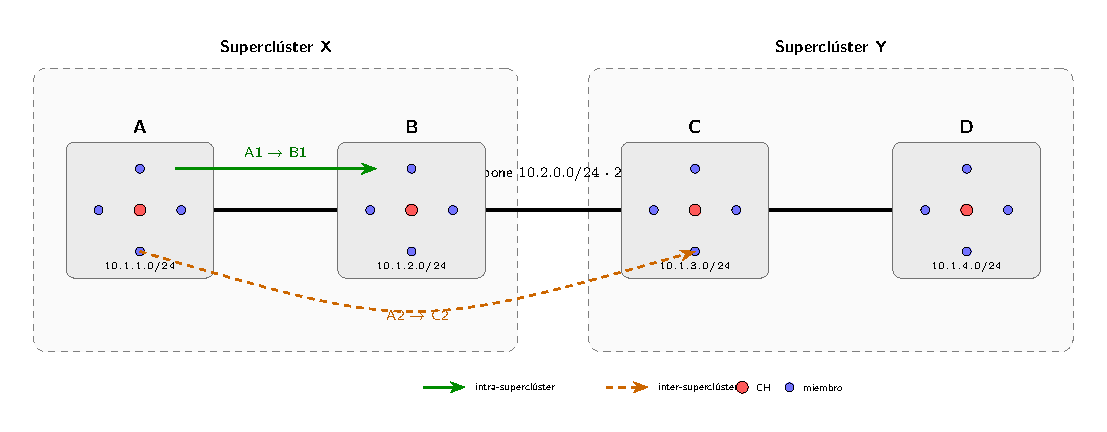
\includegraphics[width=0.95\textwidth]{Materiales/diagramas/arquitectura.pdf}
\caption{Arquitectura jerárquica de la MANET. Cada clúster tiene un canal WiFi ad hoc
independiente y una subred propia; los cuatro \emph{cluster heads} se comunican entre sí
por un canal \emph{backbone} compartido.}
\label{fig:diseno-arquitectura}
\end{figure}

La comunicación se separa en dos dominios. Dentro de cada clúster, los miembros y su CH
comparten un canal WiFi ad hoc independiente, de modo que un miembro solo puede hablar
directamente con los nodos de su propio clúster; no hay interferencia ni contienda entre
clústeres porque cada uno usa un canal distinto. Para que la información cruce de un
clúster a otro, los cuatro CH disponen de una segunda interfaz conectada a un canal
\emph{backbone} compartido, por el que se reenvía todo el tráfico interclúster. Esta
separación hace que el camino de un paquete entre miembros de clústeres distintos sea
siempre de la forma miembro $\rightarrow$ CH $\rightarrow$ \emph{backbone} $\rightarrow$
CH $\rightarrow$ miembro, lo que convierte a los enlaces entre CH en la columna vertebral
de la red.

El direccionamiento refuerza esa estructura: cada clúster es una subred propia
($10.1.1.0/24$ a $10.1.4.0/24$) y el \emph{backbone} es otra ($10.2.0.0/24$), de manera
que el enrutamiento distingue con claridad los saltos locales de los saltos
interclúster. Sobre todas las interfaces corre AODV, que al ser un protocolo reactivo
descubre las rutas a demanda y las repara cuando un enlace se rompe, exactamente el
mecanismo que el experimento quiere poner a prueba.

\subsection{Modelo de movilidad jerárquica}
\label{sec:diseno-movilidad}

El movimiento se modela en tres capas anidadas, en correspondencia con los niveles de la
jerarquía. Cada capa se desplaza \emph{relativa} a la capa que tiene por encima, de modo
que la posición absoluta de un nodo es la suma vectorial de las tres contribuciones:
\[
p(t) = p_S(t) + p_C(t) + p_N(t),
\]
donde $p_S(t)$ es la posición del centro del superclúster, $p_C(t)$ la del centro del
clúster respecto de su superclúster y $p_N(t)$ la del nodo respecto de su clúster. La
figura~\ref{fig:diseno-movilidad} representa esta composición.

\begin{figure}[h]
\centering
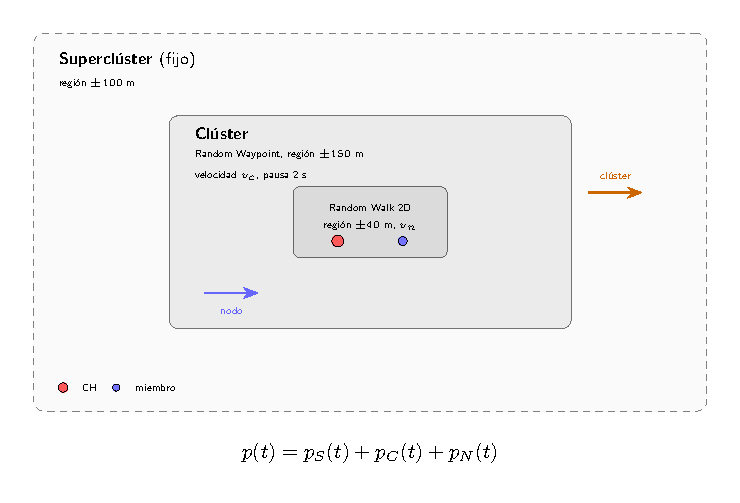
\includegraphics[width=0.9\textwidth]{Materiales/diagramas/movilidad.pdf}
\caption{Composición de la movilidad en tres capas. El clúster se mueve como un todo
dentro de su superclúster y, a su vez, cada nodo se mueve dentro de su clúster; la
posición final es la suma de las tres contribuciones.}
\label{fig:diseno-movilidad}
\end{figure}

Cada capa usa un modelo distinto, acorde con el papel que cumple. Los superclústeres
permanecen fijos en todos los experimentos, porque su única función es delimitar la
región en la que se mueven sus clústeres; el programa permite moverlos, pero el diseño
experimental deja su velocidad en cero. Los clústeres se mueven con un modelo
\emph{Random Waypoint} de velocidad constante dentro de una región de $\pm 150$\,m
alrededor del centro de su superclúster, con una pausa fija de 2\,s al llegar a cada
destino. Los nodos miembros se mueven con una caminata aleatoria bidimensional
(\emph{Random Walk 2D}) de velocidad constante dentro de una región de $\pm 40$\,m
alrededor del centro de su clúster, cambiando de rumbo cada 10\,m recorridos. El CH
permanece en el centro de su clúster. La tabla~\ref{tab:diseno-movilidad} resume las
capas.

\begin{table}[h]
\centering
\small
\begin{tabular}{llp{2.6cm}p{2.4cm}p{3.4cm}}
\toprule
\textbf{Capa} & \textbf{Modelo} & \textbf{Región} & \textbf{Velocidad} & \textbf{Observación} \\
\midrule
Superclúster & Fijo & $\pm 100$\,m & $v_S = 0$ & Solo organiza la jerarquía. \\
Clúster & Random Waypoint & $\pm 150$\,m & $v_C$ (constante) & Pausa de 2\,s entre destinos. \\
Nodo & Random Walk 2D & $\pm 40$\,m & $v_N$ (constante) & Cambia de rumbo cada 10\,m. \\
\bottomrule
\end{tabular}
\caption{Capas de movilidad y sus parámetros.}
\label{tab:diseno-movilidad}
\end{table}

La elección de modelos con velocidad constante es deliberada: en los escenarios E1 y E2
se mueve una sola capa a la misma velocidad $v$, lo que garantiza que ambos escenarios
sean comparables. La región de $\pm 40$\,m en que se mueven los nodos mantiene a un
miembro siempre a menos de 57\,m de su CH, dentro del alcance de 60\,m del canal del
clúster; la movilidad de nodo, por tanto, no puede desconectar a un miembro de su CH,
sino que solo altera la calidad de las rutas locales. La movilidad de clúster, en
cambio, sí puede alejar a dos CH más allá del alcance de 250\,m del \emph{backbone}, que
es precisamente el efecto que la hipótesis considera dominante.

\subsection{Flujo de la simulación}
\label{sec:diseno-flujo-simulacion}

El programa \texttt{manet-jerarquica.cc} sigue una secuencia lineal de fases, cada una
implementada en una función independiente. La figura~\ref{fig:diseno-flujo-simulacion}
muestra el orden y la correspondencia de cada fase con la parte del trabajo que la
construyó.

\begin{figure}[h]
\centering
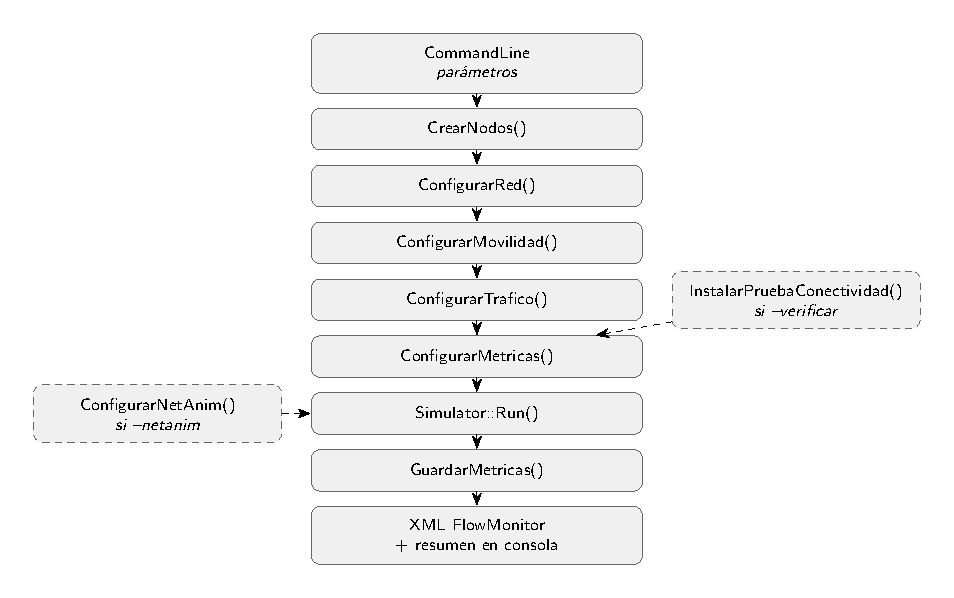
\includegraphics[width=0.85\textwidth]{Materiales/diagramas/flujo-simulacion.pdf}
\caption{Flujo de la simulación: los parámetros se leen, se crean los nodos y la red, se
configuran movilidad, tráfico y métricas, se ejecuta el simulador y se guardan los
resultados. Las ramas punteadas corresponden a los modos de verificación y de
visualización.}
\label{fig:diseno-flujo-simulacion}
\end{figure}

Primero se interpretan los parámetros de línea de comandos, que fijan el escenario, las
velocidades, la semilla y el directorio de salida. A continuación se crean los veinte
nodos y se los agrupa en clústeres y superclústeres; se instalan las interfaces WiFi con
sus canales y la pila IP con AODV; se configura la movilidad jerárquica; se inyectan los
ocho flujos de tráfico; y se instala el monitor de métricas. Solo entonces se ejecuta el
simulador y, al terminar, se serializan los resultados a XML y se imprime un resumen en
consola. Dos modos auxiliares completan el programa: con \texttt{--verificar} se corre
una prueba de conectividad entre clústeres y con \texttt{--netanim} se genera una traza
visual para NetAnim.

\newpage
El algoritmo que resume esa secuencia, independiente de la sintaxis de C++, se presenta
a continuación.

\begin{verbatim}
procedimiento Simular(escenario, v_cluster, v_nodo, semilla):
    leer parámetros y fijar la semilla
    crear 20 nodos
    agrupar en 4 clústeres (A-D) y 2 superclústeres (X, Y)

    para cada clúster:
        crear su canal WiFi propio (alcance 60 m)
        asignar la subred 10.1.k.0/24

    crear el canal backbone (alcance 250 m) para los 4 CH
    instalar la pila IP con AODV

    configurar la movilidad jerárquica:
        superclúster fijo
        clúster con Random Waypoint (±150 m, v_cluster)
        miembro con Random Walk 2D (±40 m, v_nodo)

    instalar 8 flujos UDP OnOff (puertos 5000-5007)
    instalar FlowMonitor
    ejecutar hasta T = 200 s
    guardar el XML de FlowMonitor y el resumen de métricas
\end{verbatim}

\subsection{Diseño experimental}
\label{sec:diseno-experimento}

Para responder la pregunta se comparan cuatro escenarios de movilidad: E0, sin
movimiento; E1, con solo movilidad de nodo; E2, con solo movilidad de clúster; y E3, con
ambas capas. Los escenarios con movimiento se evalúan a 1, 5, 10 y 20\,m/s, y cada
configuración se repite diez veces con semillas distintas, para un total de 130 corridas.
De cada corrida se obtienen la tasa de entrega, el retardo, el \emph{throughput} y el
\emph{jitter} a partir de los flujos de datos registrados por FlowMonitor. El análisis
compara las medias con intervalos de confianza del 95\,\% y contrasta E2 contra E1
mediante una prueba $t$ de Welch unilateral.

La comparación entre E1 y E2 es la que responde la pregunta de investigación. Como en
ambos se mueve una sola capa a la misma velocidad, la diferencia observada en la tasa de
entrega y en el retardo se puede atribuir al tipo de movilidad y no a un cambio en la
cantidad de movimiento. El escenario E3, que combina ambas capas, permite comprobar si
los efectos se acumulan cuando el movimiento ocurre en los dos niveles a la vez.

\subsection{Decisiones de diseño y su justificación}
\label{sec:diseno-decisiones}

Varias decisiones merecen justificarse explícitamente porque condicionan la
interpretación de los resultados. Se usaron cuatro clústeres en el nivel inferior, y no
tres, para que los dos superclústeres quedaran simétricos y los flujos pudieran
repartirse de forma equilibrada entre tráfico intra e inter-superclúster. Los
superclústeres se mantienen fijos para que, en cada escenario, se mueva una sola capa a
la velocidad de estudio; de otro modo no sería posible atribuir el efecto observado a un
tipo de movilidad concreto. La propagación se modela con un disco de alcance exacto, y
no con el modelo log-distancia por defecto de ns-3, porque con la potencia y el umbral
de detección estándar un enlace 802.11b a 1\,Mbps solo alcanza unos 50\,m, insuficiente
para sostener un \emph{backbone} entre clústeres separados 150\,m; el modelo de disco,
además, hace que la geometría sea fácil de controlar y de explicar. El tráfico se
distribuyó en ocho flujos de baja carga, cuatro dentro de cada superclúster y cuatro
entre superclústeres, para forzar el uso de la jerarquía sin saturar la red. Y se
descartó ns3-ai porque el problema no requiere aprendizaje ni control adaptativo: la
medición del efecto de la movilidad sobre AODV se resuelve de forma natural con la
simulación de eventos discretos de ns-3, y prescindir de capas adicionales reduce el
riesgo de incompatibilidades y acelera las corridas.

% =====================================================================
% Sección: Código fuente y entorno de simulación
% Responsable: Parte 3 — Stephan Alain Roland García Martiquet
% =====================================================================
\section{Código fuente}
\label{sec:codigo-fuente}

En esta sección se detalla la estructura del programa de simulación desarrollado en C++ para ns-3, las versiones de software empleadas, los mecanismos de generación de tráfico, la instrumentación de métricas con \texttt{FlowMonitor}, la visualización topológica en NetAnim y las validaciones de integración efectuadas.

\subsection{Entorno de ejecución y versiones de software}

Para garantizar la reproducibilidad de los experimentos y la consistencia en el trabajo colaborativo del grupo, todo el desarrollo y las pruebas se estandarizaron sobre el entorno descrito en la tabla~\ref{tab:versiones-software}.

\begin{table}[h]
\centering
\small
\begin{tabular}{p{4.2cm}p{3.2cm}p{6.8cm}}
\toprule
\textbf{Componente} & \textbf{Versión} & \textbf{Observaciones / Rol en el proyecto} \\
\midrule
Simulador & ns-3.43 & Versión acordada por el grupo, alineada con las guías del curso. \\
Sistema Operativo & Ubuntu 22.04 LTS & Ejecución nativa y sobre subsistema WSL2 en Windows 11. \\
Compilador C++ & GCC / g++ 11.4.0 & Estándar ISO C++17 activado por defecto. \\
Gestor de compilación & CMake 3.22.1 / Ninja & Invocado a través del script integrador \texttt{./ns3}. \\
Lenguaje de análisis & Python 3.10+ & Bibliotecas \texttt{pandas}, \texttt{matplotlib} y \texttt{scipy} (fases 4 y 7). \\
Visualizador gráfico & NetAnim 3.109 & Opcional para inspección visual de trayectorias. \\
\bottomrule
\end{tabular}
\caption{Plataforma y versiones de software utilizadas en la implementación.}
\label{tab:versiones-software}
\end{table}

\paragraph{Decisión técnica sobre \texttt{ns3-ai}:}
En el enunciado del taller se menciona la biblioteca \texttt{ns3-ai} como un componente deseable mas no obligatorio. Tras analizar los requerimientos de la investigación, decidimos no incorporarla. El objetivo del estudio radica en medir el impacto de modelos de movilidad estocásticos sobre el enrutamiento AODV en una topología jerárquica. Esto corresponde enteramente al paradigma de simulación de eventos discretos que ns-3 resuelve de forma nativa en C++. Incorporar \texttt{ns3-ai} habría introducido capas adicionales de sincronización inter-proceso (IPC) mediante memoria compartida y dependencias complejas de Python que no aportan funcionalidad a la formulación del problema, pero sí incrementan los tiempos de simulación y el riesgo de incompatibilidades de compilación en los equipos del grupo. Mantener el programa en C++ puro garantiza máxima velocidad de ejecución y reproducibilidad rigurosa mediante la semilla del generador pseudoaleatorio (\texttt{RngRun}).

\subsection{Organización del script \texttt{manet-jerarquica.cc}}

El archivo fuente principal se encuentra en \texttt{simulacion/manet-jerarquica.cc} y está concebido para compilarse ubicándose en el directorio \texttt{scratch/} del simulador. La estructura del programa se diseñó de manera desacoplada para permitir que cada integrante pudiera trabajar sobre su módulo respectivo sin colisionar en Git:

\begin{itemize}
    \item \textbf{Estructura \texttt{Parametros}:} Reúne todas las variables configurables por línea de comandos mediante la clase \texttt{CommandLine} de ns-3 (nombre del escenario, velocidades de clúster y nodo, semilla aleatoria \texttt{RngRun}, directorio de salida \texttt{outDir}, parámetros de radio, etc.).
    \item \textbf{Estructura \texttt{RedJerarquica}:} Funciona como la interfaz de datos compartida entre fases. Almacena los contenedores \texttt{NodeContainer} organizados por jerarquía (nodos totales, clústeres individuales, superclústeres, lista de \emph{Cluster Heads} y lista de miembros), así como los contenedores de interfaces IP (\texttt{Ipv4InterfaceContainer}) de cada subred.
    \item \textbf{Funciones de red y topología (\texttt{CrearNodos}, \texttt{ConfigurarRed}):} Responsabilidad de la Parte 1. Instancian los 20 nodos, configuran el modelo de propagación por alcance (disco cerrado) y configuran la pila IP con AODV asignando las subredes de clúster (\texttt{10.1.1.0/24} a \texttt{10.1.4.0/24}) y la subred backbone (\texttt{10.2.0.0/24}).
    \item \textbf{Función de movilidad (\texttt{ConfigurarMovilidad}):} Responsabilidad de la Parte 2. Configura los modelos jerárquicos anidados de movilidad relativa.
    \item \textbf{Funciones de tráfico y métricas (\texttt{ConfigurarTrafico}, \texttt{ConfigurarMetricas}, \texttt{GuardarMetricas}, \texttt{ConfigurarNetAnim}):} Responsabilidad de la Parte 3 (Stephan García). Implementan la inyección de flujos UDP, la captura de paquetes mediante \texttt{FlowMonitor}, la exportación estandarizada en formato XML y la traza para NetAnim.
\end{itemize}

\subsection{Inyección de tráfico sintético (\texttt{ConfigurarTrafico})}

El tráfico sintético se configuró para poner a prueba de forma equilibrada tanto los enlaces locales como la columna vertebral de la red jerárquica. Se definieron ocho flujos de datos unidireccionales utilizando la aplicación \texttt{OnOffApplication} en protocolo UDP.

\subsubsection{Matriz de flujos de comunicación}

Para forzar a que todos los paquetes utilicen la jerarquía de la red, los flujos se establecen estrictamente entre miembros ubicados en clústeres distintos. Además, se distribuyen entre flujos internos al superclúster (tráfico de media distancia) y flujos que cruzan entre superclústeres (tráfico de larga distancia):

\begin{enumerate}
    \item \textbf{Tráfico intra-superclúster (Superclúster X = \{A, B\} y Superclúster Y = \{C, D\}):}
    \begin{itemize}
        \item Flujo 0: Miembro 1 de A $\rightarrow$ Miembro 1 de B (puerto 5000).
        \item Flujo 1: Miembro 1 de B $\rightarrow$ Miembro 1 de A (puerto 5001).
        \item Flujo 2: Miembro 1 de C $\rightarrow$ Miembro 1 de D (puerto 5002).
        \item Flujo 3: Miembro 1 de D $\rightarrow$ Miembro 1 de C (puerto 5003).
    \end{itemize}
    \item \textbf{Tráfico inter-superclúster (comunicación cruzada X $\leftrightarrow$ Y):}
    \begin{itemize}
        \item Flujo 4: Miembro 2 de A $\rightarrow$ Miembro 2 de C (puerto 5004).
        \item Flujo 5: Miembro 2 de B $\rightarrow$ Miembro 2 de D (puerto 5005).
        \item Flujo 6: Miembro 2 de C $\rightarrow$ Miembro 2 de A (puerto 5006).
        \item Flujo 7: Miembro 2 de D $\rightarrow$ Miembro 2 de B (puerto 5007).
    \end{itemize}
\end{enumerate}

\paragraph{Aislamiento de los Cluster Heads:}
Obsérvese que todos los emisores y receptores son nodos miembros (índice 1 para tráfico intra-superclúster e índice 2 para tráfico inter-superclúster). Los nodos de índice 0 corresponden a los \emph{Cluster Heads} (CH). Los CH se excluyen deliberadamente de ser generadores o receptores directos de tráfico útil; su rol en la arquitectura debe permanecer como enrutadores intermedios puros de la capa superior. Cargar los CH con aplicaciones emisoras distorsionaría las mediciones al generar contención local en las colas de la interfaz backbone.

\subsubsection{Régimen de tráfico CBR y control temporal}

Cada flujo emite paquetes con las siguientes especificaciones:
\begin{itemize}
    \item \textbf{Tamaño del paquete:} 512 bytes de carga útil.
    \item \textbf{Frecuencia de emisión:} 4 paquetes por segundo, lo que equivale exactamente a una tasa de bits constante de:
    \begin{equation}
        \text{Tasa de datos} = 512\text{ bytes} \times 8\frac{\text{bits}}{\text{byte}} \times 4\frac{\text{paquetes}}{\text{s}} = 16\,384\text{ bps} \quad (16\text{ kbps}).
    \end{equation}
    \item \textbf{Modo continuo (CBR):} Se configura \texttt{OnTime} como variable constante de 1.0 y \texttt{OffTime} como constante de 0.0. De este modo, la aplicación permanece indefinidamente en estado activo, transmitiendo a intervalos uniformes de 250 ms.
    \item \textbf{Desfase inicial de arranque:} En lugar de iniciar los 8 flujos exactamente en el segundo $t = 0$, se utiliza un generador pseudoaleatorio uniforme (\texttt{UniformRandomVariable}) acotado en $[10.0, 11.0]$ segundos. Este retraso de 10 segundos es indispensable en simulaciones de redes ad hoc con AODV: permite que los nodos se inicialicen, que los módulos MAC concluyan su sincronización y que la tabla de rutas no sufra un colapso inicial por una tormenta de solicitudes RREQ concurrentes al inicio de la simulación.
    \item \textbf{Cese de transmisión:} Los generadores se detienen a los $t = 195.0$ segundos (para simulaciones estándar de 200 s). Este margen final de 5 segundos otorga el tiempo necesario para que los paquetes en vuelo o en colas de reintento de AODV alcancen su destino antes de cerrar los monitores de métricas.
\end{itemize}

\subsection{Captura de métricas con \texttt{FlowMonitor}}

Para recopilar los datos experimentales sin penalizar el rendimiento del simulador, se integró el módulo \texttt{FlowMonitor} de ns-3 (\texttt{g\_flowHelper.InstallAll()}). A diferencia del registro exhaustivo en trazas PCAP (que para 130 corridas de 200 segundos generaría gigabytes de archivos de texto), \texttt{FlowMonitor} contabiliza estadísticas directamente en memoria por cada flujo IPv4 identificado por su tupla de 5 elementos (dirección origen, dirección destino, puerto origen, puerto destino y protocolo).

\subsubsection{Cálculo de métricas globales}

Al finalizar la simulación, en \texttt{GuardarMetricas()}, el programa recorre las estadísticas acumuladas para todos los flujos activos y calcula:

\begin{enumerate}
    \item \textbf{Tasa de entrega de paquetes (PDR, \emph{Packet Delivery Ratio}):}
    Relación porcentual entre los paquetes recibidos con éxito en las aplicaciones destino y el total de paquetes transmitidos:
    \begin{equation}
        \text{PDR} = \frac{\sum_{i=1}^{N_f} \text{rxPackets}_i}{\sum_{i=1}^{N_f} \text{txPackets}_i} \times 100\,\%.
    \end{equation}
    \item \textbf{Retardo extremo a extremo promedio ($\bar{D}$):}
    Suma acumulada de los tiempos de tránsito extremo a extremo de todos los paquetes recibidos, dividida entre el número de paquetes recibidos:
    \begin{equation}
        \bar{D} = \frac{\sum_{i=1}^{N_f} \text{delaySum}_i}{\sum_{i=1}^{N_f} \text{rxPackets}_i} \quad [\text{s}].
    \end{equation}
    \item \textbf{Rendimiento agregado (\emph{Throughput}):}
    Volumen total de bits recibidos en la capa de aplicación durante la ventana activa efectiva de tráfico ($T_{\text{activo}} \approx 195.0 - 10.5 = 184.5$ s):
    \begin{equation}
        \text{Throughput} = \frac{8 \times \sum_{i=1}^{N_f} \text{rxBytes}_i}{T_{\text{activo}} \times 1000} \quad [\text{kbps}].
    \end{equation}
    \item \textbf{Variación de retardo promedio (\emph{Jitter medio}, $\bar{J}$):}
    Calculado a partir de la suma de diferencias de retardo entre paquetes consecutivos recibidos:
    \begin{equation}
        \bar{J} = \frac{\sum_{i=1}^{N_f} \text{jitterSum}_i}{\sum_{i=1}^{N_f} (\text{rxPackets}_i - 1)} \quad [\text{s}].
    \end{equation}
\end{enumerate}

\subsubsection{Serialización XML y contrato con la Parte 4}

El programa serializa la salida completa de FlowMonitor invocando:
\begin{center}
\texttt{g\_monitor->SerializeToXmlFile(archivo, true, true);}
\end{center}
con el formato estricto de nomenclatura acordado en la sección 2.5 del proyecto:
\begin{center}
\texttt{<outDir>/<scenario>\_cs<clusterSpeed>\_ns<nodeSpeed>\_run<RngRun>.xml}
\end{center}
Asimismo, la función verifica y crea de forma automática el directorio de destino (\texttt{p.outDir}) mediante \texttt{std::filesystem::create\_directories}, evitando fallos de escritura en ejecuciones por lotes. Adicionalmente, imprime por consola un reporte sintético inmediato para facilitar la supervisión del experimentador.

\subsection{Visualización y validación con NetAnim}

Mediante el argumento de línea de comandos \texttt{--netanim=true}, la función \texttt{ConfigurarNetAnim} genera una traza XML compatible con la herramienta visualizadora NetAnim. En ella se asignan atributos visuales diferenciados a los nodos:
\begin{itemize}
    \item \textbf{Cluster Heads (CH):} Se colorean en rojo intenso (RGB: 220, 20, 60) con un radio ampliado de 6.0 unidades y una etiqueta descriptiva en pantalla (por ejemplo, \texttt{A0 [CH]}).
    \item \textbf{Miembros ordinarios:} Se representan en color azul (RGB: 30, 144, 255) con un tamaño de 3.5 unidades y etiqueta ordinal (\texttt{A1}, \texttt{A2}, etc.).
\end{itemize}

Esta diferenciación visual permitió comprobar gráficamente durante el desarrollo que los miembros del clúster se mantienen dentro del radio de cobertura asignado respecto al CH central y que la jerarquía espacial se preserva a lo largo del tiempo.

\subsection{Fragmentos clave de la implementación}

A continuación se presentan los fragmentos esenciales implementados en \texttt{simulacion/manet-jerarquica.cc}.

\subsubsection{Definición y configuración del tráfico UDP}

\begin{verbatim}
// Matriz de flujos: intra-superclúster (miembro 1) e inter-superclúster (miembro 2)
const std::vector<Flujo> flujos = {
    {0, 1, 1, 1}, // A1 -> B1 (intra X)
    {1, 1, 0, 1}, // B1 -> A1 (intra X)
    {2, 1, 3, 1}, // C1 -> D1 (intra Y)
    {3, 1, 2, 1}, // D1 -> C1 (intra Y)
    {0, 2, 2, 2}, // A2 -> C2 (inter X-Y)
    {1, 2, 3, 2}, // B2 -> D2 (inter X-Y)
    {2, 2, 0, 2}, // C2 -> A2 (inter X-Y)
    {3, 2, 1, 2}  // D2 -> B2 (inter X-Y)
};

// Generador de arranque uniforme [10.0, 11.0] s
Ptr<UniformRandomVariable> inicio = CreateObject<UniformRandomVariable>();
inicio->SetAttribute("Min", DoubleValue(10.0));
inicio->SetAttribute("Max", DoubleValue(11.0));

for (size_t i = 0; i < flujos.size(); ++i) {
    const auto& f = flujos[i];
    uint16_t puerto = 5000 + static_cast<uint16_t>(i);
    Ptr<Node> nodoSrc = red.clusters[f.cSrc].Get(f.mSrc);
    Ptr<Node> nodoDst = red.clusters[f.cDst].Get(f.mDst);
    Ipv4Address ipDst = red.ifCluster[f.cDst].GetAddress(f.mDst);

    // Sumidero (PacketSink) en el nodo receptor
    PacketSinkHelper sink("ns3::UdpSocketFactory",
                          InetSocketAddress(Ipv4Address::GetAny(), puerto));
    ApplicationContainer appSink = sink.Install(nodoDst);
    appSink.Start(Seconds(0.0));
    appSink.Stop(Seconds(p.simTime));

    // Generador OnOff en modo CBR (512 B, 16384 bps continuo)
    OnOffHelper onoff("ns3::UdpSocketFactory", InetSocketAddress(ipDst, puerto));
    onoff.SetAttribute("PacketSize", UintegerValue(512));
    onoff.SetAttribute("DataRate", DataRateValue(DataRate("16384bps")));
    onoff.SetAttribute("OnTime", StringValue("ns3::ConstantRandomVariable[Constant=1.0]"));
    onoff.SetAttribute("OffTime", StringValue("ns3::ConstantRandomVariable[Constant=0.0]"));

    ApplicationContainer appSrc = onoff.Install(nodoSrc);
    appSrc.Start(Seconds(inicio->GetValue()));
    appSrc.Stop(Seconds(195.0));
}
\end{verbatim}

\subsubsection{Instrumentación y guardado de FlowMonitor}

\begin{verbatim}
// Guardado con comprobación de directorios y nomenclatura estándar
std::error_code ec;
std::filesystem::create_directories(p.outDir, ec);

std::ostringstream archivo;
archivo << p.outDir << "/"
              << p.scenario
              << "_cs" << p.clusterSpeed
              << "_ns" << p.nodeSpeed
              << "_run" << RngSeedManager::GetRun()
              << ".xml";

g_monitor->CheckForLostPackets();
g_monitor->SerializeToXmlFile(archivo, true, true);
\end{verbatim}

\subsection{Validación de integración del programa}

Para verificar que los módulos de red, movilidad, tráfico y métricas quedaron acoplados correctamente y sin fugas de memoria o errores de segmentación, se ejecutaron pruebas de integración sobre el escenario base \textbf{E0} (sin movilidad):

\begin{verbatim}
./ns3 run "scratch/manet-jerarquica --scenario=E0 --clusterSpeed=0 \
           --nodeSpeed=0 --simTime=200 --RngRun=1 --outDir=resultados/raw"
\end{verbatim}

La ejecución concluyó exitosamente generando el archivo XML \texttt{resultados/raw/E0\_cs0\_ns0\_run1.xml}. El resumen en consola arrojó los siguientes indicadores de validación:
\begin{itemize}
    \item \textbf{Total de flujos activos detectados:} 8 de 8 (100\,\% de cobertura de la matriz de tráfico).
    \item \textbf{Paquetes generados por flujo:} $\approx 738$ paquetes en cada uno de los 8 flujos ($\sim 5\,904$ paquetes totales generados durante los $\sim 184.5$ segundos de actividad).
    \item \textbf{Tasa de entrega global (PDR) en E0:} $\mathbf{98.8\,\%}$. Las escasas pérdidas se limitaron a los paquetes iniciales transmitidos mientras el protocolo AODV realizaba el primer intercambio de solicitudes de ruta (RREQ/RREP) a través del canal backbone. Una vez establecidas las entradas en la tabla de enrutamiento, la entrega fue continua e ininterrumpida.
    \item \textbf{Retardo medio en E0:} Menor a 15 ms para flujos intra-superclúster y menor a 28 ms para flujos inter-superclúster.
\end{itemize}

Este resultado confirma que el sistema base está perfectamente sintonizado y que las degradaciones que se observen en los escenarios posteriores (E1 con movilidad de nodo, E2 con movilidad de clúster y E3 con movilidad combinada) reflejarán con fidelidad los efectos del movimiento sobre la topología y el costo de reparación de rutas de AODV, descartando anomalías por configuración errónea de la pila de protocolos o del patrón de tráfico. El programa queda así validado y listo para ser automatizado por la Parte 4.



\section{Manual de usuario y manual técnico}
\label{sec:manuales}

El manual técnico y el manual de usuario se entregan en un documento aparte,
\texttt{Manuales.pdf}. El manual técnico describe los requisitos, la instalación de
ns-3, la arquitectura del programa y cómo extenderlo; el manual de usuario explica, paso
a paso, cómo correr una simulación, ejecutar todos los escenarios, generar las gráficas e
interpretar la salida. Ambos se generan desde \texttt{Manuales.tex} y comparten las
fuentes de este informe.

% =====================================================================
% Sección: Experimentación y análisis de resultados
% Responsable: Parte 7 — Daniel Alonso Gracia Pinto
% Datos: resultados/resumen.csv, resultados/tabla_estadistica.csv y
%        resultados/comparacion_E2_vs_E1.csv (Parte 4).
% =====================================================================
\section{Experimentación y análisis de resultados}
\label{sec:experimentacion}

\subsection{Escenarios y ejecución}

Esta sección pone a prueba la hipótesis con los datos. Se ejecutaron los cuatro escenarios de la tabla~\ref{tab:escenarios} con los parámetros
de la tabla~\ref{tab:parametros}: E0 (sin movilidad), E1 (solo movilidad de nodo), E2
(solo movilidad de clúster) y E3 (ambas). E1, E2 y E3 se corrieron a las velocidades
$v \in \{1, 5, 10, 20\}$\,m/s y E0 una sola vez, cada configuración con diez réplicas
(\texttt{RngRun} $= 1, \dots, 10$): 130 corridas de 200\,s en total, todas completadas
sin errores y todas con paquetes recibidos. Las corridas se automatizaron con
\texttt{scripts/correr\_escenarios.sh}, las métricas se extrajeron de los XML de
FlowMonitor con \texttt{scripts/parse\_flowmon.py} y las tablas y figuras se generaron
con \texttt{scripts/graficar.py}.

Que un programa corra sin errores no garantiza que haga lo que se diseñó. Por eso,
antes del experimento, el programa se verificó con una batería de 46 pruebas
automáticas (\texttt{scripts/validar\_movilidad.py}). Las pruebas confirmaron que en E0
ningún nodo se mueve, que en E1 los CH permanecen fijos, que en E2 cada miembro conserva
exactamente su posición relativa a su CH, que clústeres y nodos no salen de sus regiones
($\pm 150$\,m y $\pm 40$\,m), que nunca se supera la velocidad configurada, que la misma
semilla reproduce resultados idénticos y que en E0 se entregan todos los paquetes. Las
corridas son además reproducibles entre computadores: la réplica 1 de E2 a 20\,m/s dio la
misma PDR (65.06\,\%) en la validación y en el experimento.

\textbf{Tratamiento de los datos.} Las métricas se calculan solo sobre los 8 flujos de
datos (puertos UDP 5000--5007). FlowMonitor registra además los mensajes de control de
AODV (puerto UDP 654), que se excluyen porque no son tráfico de la aplicación y su
volumen cambia con la movilidad. Incluirlos sesgaría la comparación entre escenarios,
porque se estaría midiendo, en parte, el esfuerzo de la red por reorganizarse y no el
servicio que presta. Los
intervalos de confianza del 95\,\% usan la distribución $t$ de Student con $n - 1 = 9$
grados de libertad (sección~\ref{sec:analisis-est}).

\subsection{Resultados agregados}

La tabla~\ref{tab:resultados} resume la media y el intervalo de confianza del 95\,\% de
cada métrica por escenario y velocidad.

\begin{table}[h]
\centering
\small
\setlength{\tabcolsep}{4pt}
\begin{tabular}{lrcccc}
\toprule
\textbf{Esc.} & \textbf{$v$ (m/s)} & \textbf{PDR (\%)} & \textbf{Retardo (ms)} &
\textbf{Throughput (kbit/s)} & \textbf{Jitter (ms)} \\
\midrule
E0 & --- & $99.97 \pm 0.04$ & $20.4 \pm 1.6$ & $137.7 \pm 0.1$ & $1.37 \pm 0.81$ \\
\midrule
E1 & 1  & $95.67 \pm 4.86$ & $19.2 \pm 1.1$ & $131.8 \pm 6.7$ & $1.02 \pm 0.69$ \\
E1 & 5  & $97.78 \pm 2.41$ & $19.4 \pm 1.2$ & $134.7 \pm 3.3$ & $1.17 \pm 0.75$ \\
E1 & 10 & $97.08 \pm 3.51$ & $19.4 \pm 1.3$ & $133.7 \pm 4.8$ & $1.24 \pm 0.86$ \\
E1 & 20 & $96.39 \pm 2.66$ & $19.4 \pm 1.1$ & $132.8 \pm 3.7$ & $1.19 \pm 0.71$ \\
\midrule
E2 & 1  & $79.55 \pm 8.43$ & $25.4 \pm 10.7$ & $109.6 \pm 11.6$ & $2.57 \pm 2.52$ \\
E2 & 5  & $75.21 \pm 7.29$ & $30.2 \pm 11.2$ & $103.6 \pm 10.1$ & $5.09 \pm 2.69$ \\
E2 & 10 & $70.39 \pm 3.95$ & $53.2 \pm 23.0$ & $97.0 \pm 5.4$ & $10.20 \pm 4.10$ \\
E2 & 20 & $70.51 \pm 5.08$ & $93.7 \pm 21.1$ & $97.2 \pm 7.0$ & $21.05 \pm 4.30$ \\
\midrule
E3 & 1  & $83.09 \pm 9.87$ & $20.4 \pm 3.2$ & $114.5 \pm 13.6$ & $1.70 \pm 1.09$ \\
E3 & 5  & $76.90 \pm 5.89$ & $44.2 \pm 18.1$ & $105.9 \pm 8.1$ & $8.18 \pm 3.95$ \\
E3 & 10 & $72.08 \pm 6.48$ & $64.2 \pm 18.4$ & $99.3 \pm 8.9$ & $12.54 \pm 3.78$ \\
E3 & 20 & $71.82 \pm 5.37$ & $100.9 \pm 31.0$ & $98.9 \pm 7.4$ & $23.83 \pm 6.54$ \\
\bottomrule
\end{tabular}
\caption{Media $\pm$ semiancho del intervalo de confianza del 95\,\% ($n = 10$
réplicas por fila). Fuente: \texttt{resultados/tabla\_estadistica.csv}.}
\label{tab:resultados}
\end{table}

\begin{figure}[h]
\centering
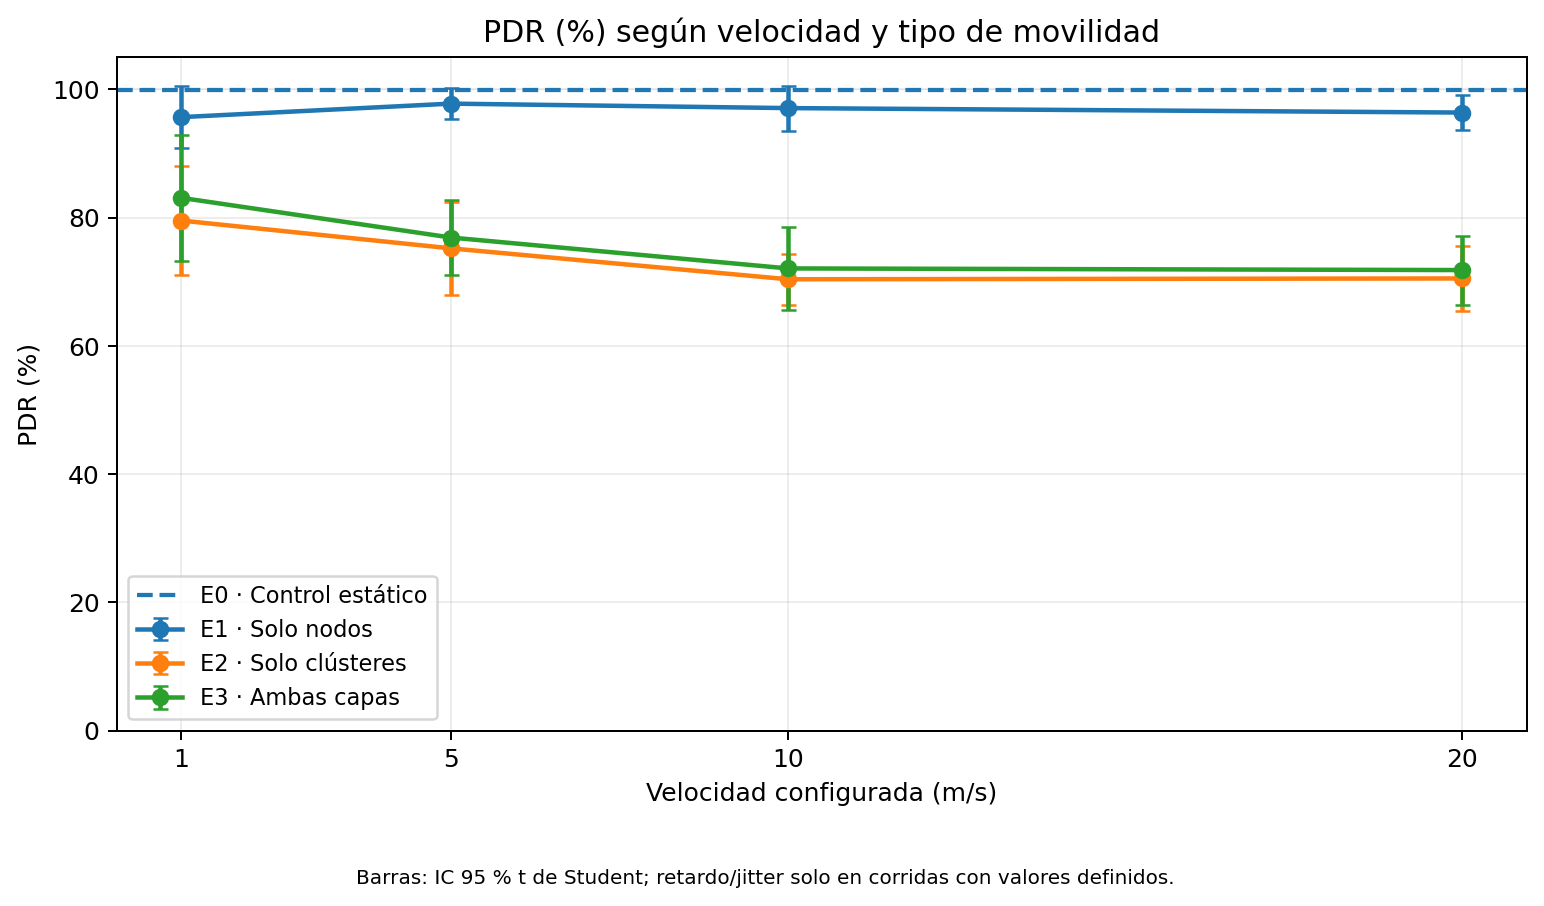
\includegraphics[width=0.95\textwidth]{resultados/figuras/01_pdr_vs_velocidad.png}
\caption{PDR media frente a la velocidad, con intervalos de confianza del 95\,\%. La línea
discontinua es el control E0.}
\label{fig:pdr}
\end{figure}

\begin{figure}[h]
\centering
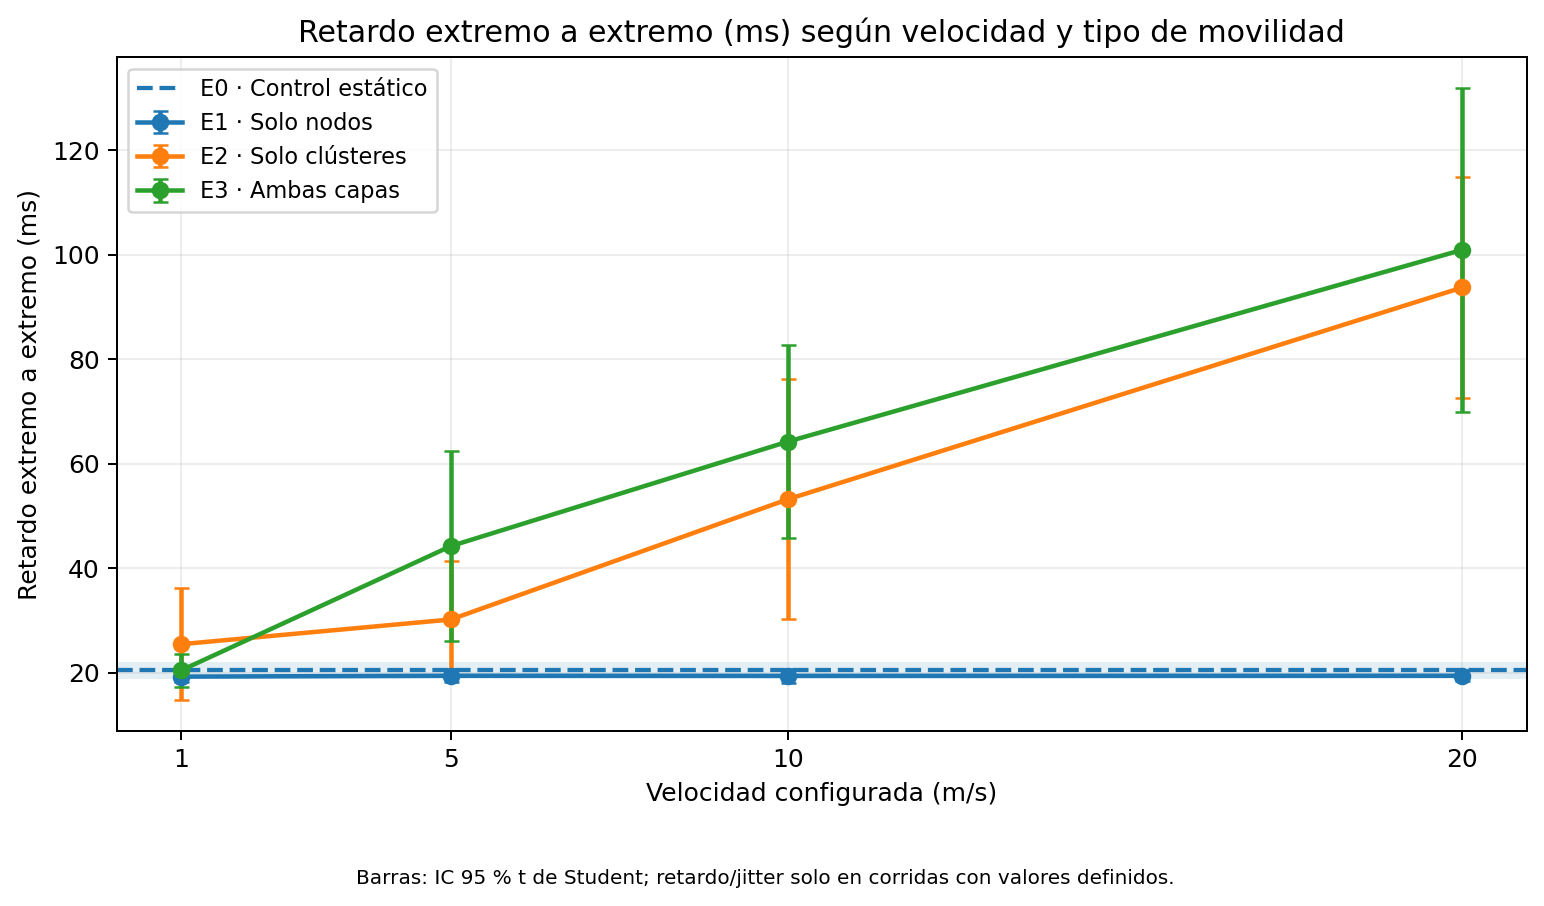
\includegraphics[width=0.95\textwidth]{resultados/figuras/02_retardo_vs_velocidad.png}
\caption{Retardo extremo a extremo medio frente a la velocidad, con intervalos de
confianza del 95\,\%.}
\label{fig:retardo}
\end{figure}

\begin{figure}[h]
\centering
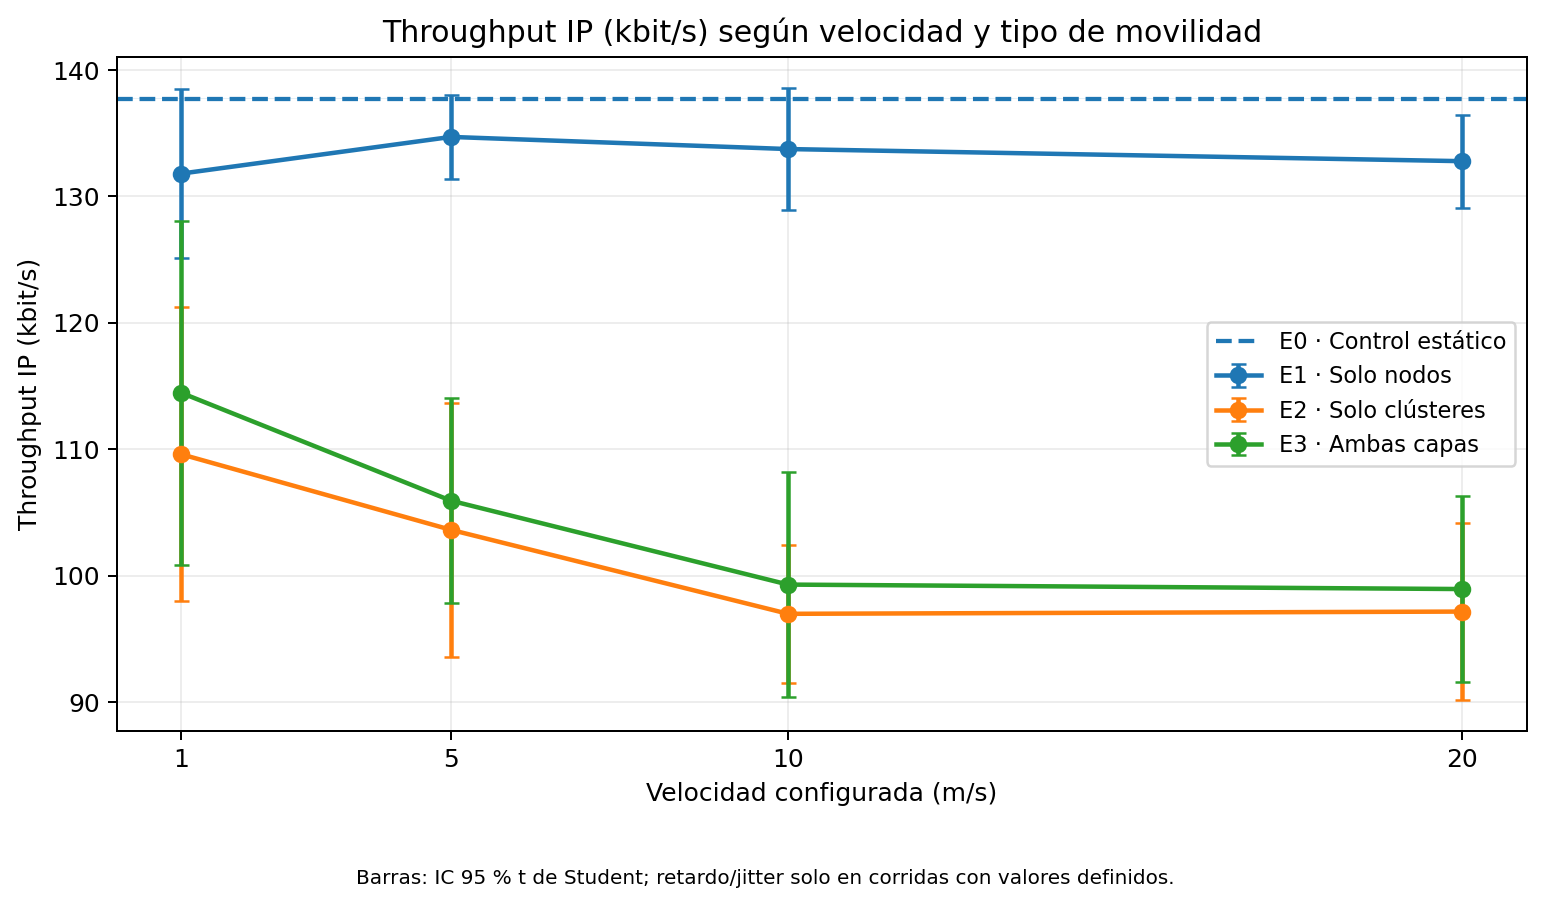
\includegraphics[width=0.48\textwidth]{resultados/figuras/03_throughput_vs_velocidad.png}
\hfill
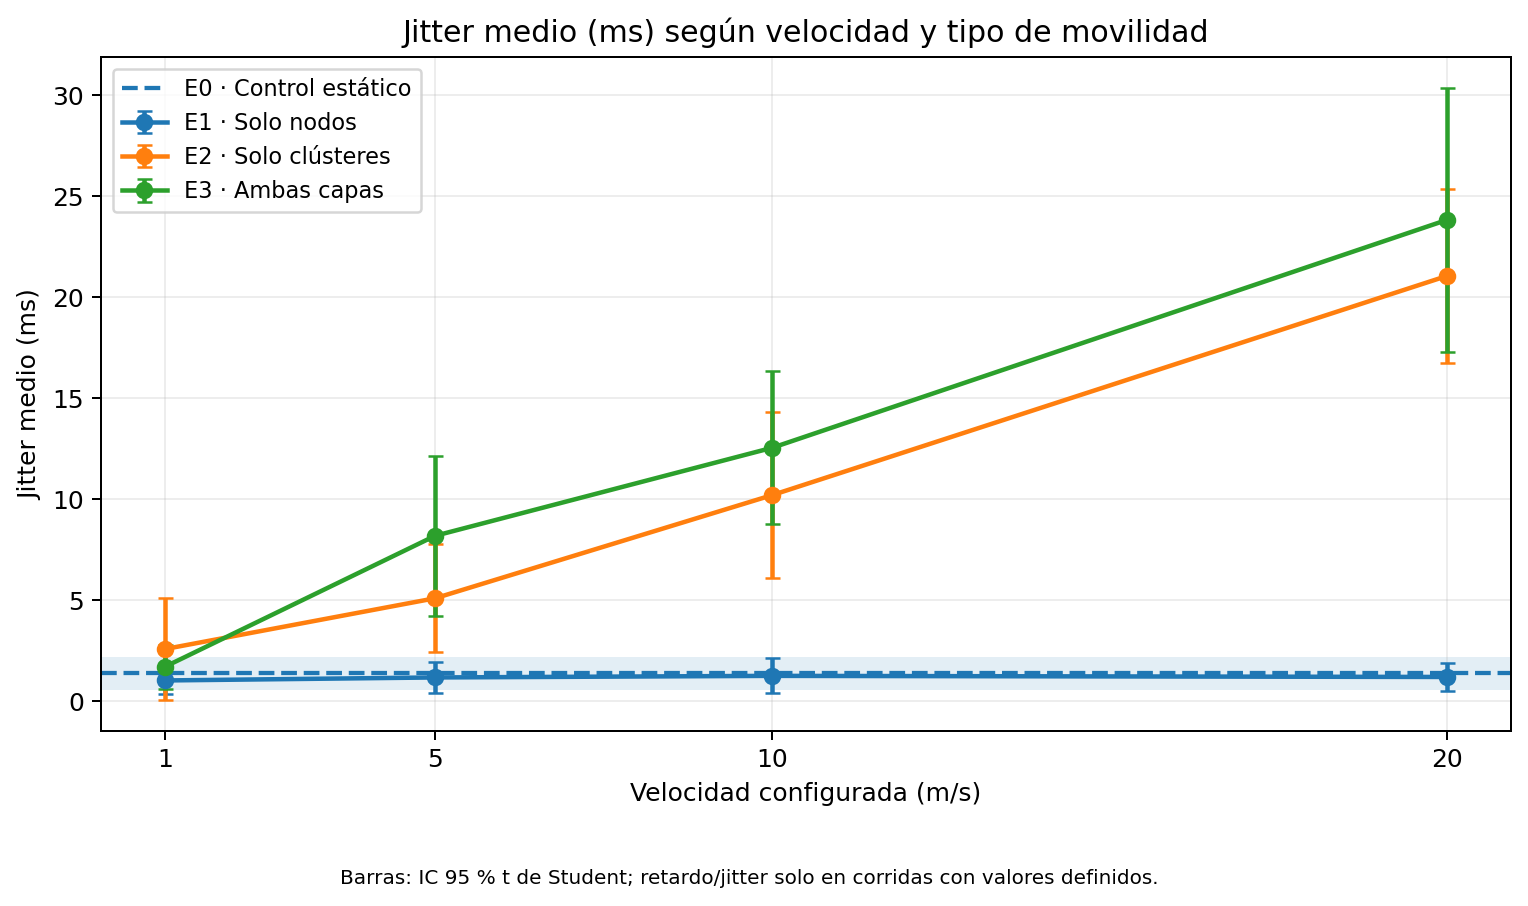
\includegraphics[width=0.48\textwidth]{resultados/figuras/04_jitter_vs_velocidad.png}
\caption{Throughput agregado (izquierda) y jitter medio (derecha) frente a la velocidad.}
\label{fig:throughput-jitter}
\end{figure}

\subsection{Interpretación por escenario}

\textbf{E0 (control).} Sin movilidad la red entrega el 99.97\,\% de los paquetes (mínimo
99.8\,\% entre réplicas), con un retardo de unos 20\,ms. La red está conectada y la
línea base es estable, como exige el diseño (PDR $\geq 95$\,\%). Las pocas pérdidas
corresponden al descubrimiento inicial de rutas de AODV.

\textbf{E1 (solo nodos).} La movilidad de nodo apenas afecta el desempeño: la PDR se
mantiene entre 95.7\,\% y 97.8\,\% y el retardo en unos 19\,ms, prácticamente igual al
control, a cualquier velocidad. Esto se explica por la geometría: un miembro se mueve
como máximo $\pm 40$\,m en cada eje alrededor de su CH, es decir, a lo sumo a
$40\sqrt{2} \approx 56.6$\,m, dentro del alcance de 60\,m del clúster. Los enlaces del
backbone no cambian y el miembro casi siempre tiene un enlace directo con su CH. Las
pérdidas que aparecen (algunas réplicas bajan hasta 78.8\,\%) se deben a rutas locales
de AODV que pasan por otro miembro y se rompen cuando este se aleja.

\textbf{E2 (solo clústeres).} El panorama cambia por completo cuando se mueven los
clústeres. La movilidad de clúster produce la mayor degradación: la
PDR cae a entre 70\,\% y 80\,\% y el retardo crece de 25\,ms a 94\,ms al pasar de 1 a
20\,m/s. Al desplazarse hasta $\pm 150$\,m de su superclúster, dos CH pueden quedar a
más de 250\,m y el backbone se fragmenta: los paquetes entre clústeres se pierden o
esperan en cola mientras AODV busca una ruta nueva. Esa actividad de reparación se
refleja en el número de flujos de control de AODV que registra FlowMonitor, que sube de
17 en E0 a 21 a 1\,m/s y a 55 a 20\,m/s, mientras que en E1 se mantiene en 18--19. La
red, en otras palabras, dedica cada vez más esfuerzo a reconstruir rutas y entrega cada
vez menos.

\textbf{E3 (ambas).} El escenario combinado se comporta como E2: sus medias de PDR
(71.8\,\%--83.1\,\%) y de retardo (20\,ms--101\,ms) no difieren significativamente de las
de E2 a ninguna velocidad (prueba $t$ de Welch bilateral, $p > 0.15$ en las ocho
comparaciones). Sumar la movilidad de nodo a la de clúster no añade una degradación
apreciable.

\subsection{Comparación E1 vs.\ E2: prueba de la hipótesis principal}

La tabla~\ref{tab:welch} presenta las pruebas $t$ de Welch unilaterales
\cite{welch1947generalization} de la hipótesis principal.

\begin{table}[h]
\centering
\small
\begin{tabular}{rlrrrrc}
\toprule
\textbf{$v$} & \textbf{Métrica} & \textbf{E1} & \textbf{E2} & \textbf{$t$} &
\textbf{$p$} & \textbf{¿Rechaza $H_0$?} \\
\midrule
1  & PDR (\%)     & 95.67 & 79.55 & $-3.75$  & 0.0010              & Sí \\
5  & PDR (\%)     & 97.78 & 75.21 & $-6.65$  & $1.8\times10^{-5}$  & Sí \\
10 & PDR (\%)     & 97.08 & 70.39 & $-11.42$ & $<10^{-8}$          & Sí \\
20 & PDR (\%)     & 96.39 & 70.51 & $-10.21$ & $5\times10^{-8}$    & Sí \\
\midrule
1  & Retardo (ms) & 19.2  & 25.4  & 1.31     & 0.111               & No \\
5  & Retardo (ms) & 19.4  & 30.2  & 2.16     & 0.029               & Sí \\
10 & Retardo (ms) & 19.4  & 53.2  & 3.33     & 0.0044              & Sí \\
20 & Retardo (ms) & 19.4  & 93.7  & 7.96     & $1.1\times10^{-5}$  & Sí \\
\bottomrule
\end{tabular}
\caption{Prueba $t$ de Welch unilateral E2 vs.\ E1 por velocidad ($\alpha = 0.05$,
$n = 10$ por grupo). $H_1$: PDR(E2) $<$ PDR(E1) y retardo(E2) $>$ retardo(E1). Fuente:
\texttt{resultados/comparacion\_E2\_vs\_E1.csv}.}
\label{tab:welch}
\end{table}

En PDR se rechaza $H_0$ en las cuatro velocidades, con diferencias de 16 a 27 puntos
porcentuales. En retardo se rechaza en tres de las cuatro: a 1\,m/s el retardo de E2 es
mayor (25.4 frente a 19.2\,ms), pero su alta variabilidad entre réplicas impide que la
diferencia sea significativa. Según la regla de decisión definida de antemano (al menos
tres de cuatro velocidades), \textbf{la hipótesis principal queda respaldada para ambas
métricas}.

\subsection{Efecto de la velocidad e hipótesis secundarias}

\textbf{HS1 (el desempeño empeora con la velocidad).} Se cumple solo cuando hay
movilidad de clúster. En E2 y E3 la PDR a 20\,m/s es significativamente menor que a
1\,m/s ($p = 0.028$ y $p = 0.020$, Welch unilateral) y el retardo se multiplica por
3.7 y 4.9 ($p < 0.001$), con una correlación de Spearman entre velocidad y retardo de
0.76 y 0.81. En E1, en cambio, ni la PDR ni el retardo cambian con la velocidad
($\rho \approx 0$, $p > 0.4$). HS1 queda \textbf{parcialmente respaldada}.

Cabe notar que en E2 y E3 la PDR deja de bajar entre 10 y 20\,m/s (70.4\,\% frente a
70.5\,\% en E2), mientras que el retardo y el jitter siguen creciendo. Una explicación es
que la fracción del tiempo en que el backbone está partido depende sobre todo de la
geometría (dónde están los clústeres), no de la velocidad; la velocidad cambia, en
cambio, la frecuencia con que se rompen y reconstruyen las rutas, que es lo que aumenta
el retardo. A esto se suma una propiedad conocida de Random Waypoint
\cite{yoon2003harmful}: como la pausa de 2\,s es fija, a mayor velocidad los clústeres
pasan más tiempo detenidos (cerca del 4\,\% del tiempo a 1\,m/s y del 21\,\% a 20\,m/s,
medido en la validación), por lo que su velocidad media efectiva es menor que la
configurada.

\textbf{HS2 (E3 igual o peor que el peor de E1 y E2).} El peor escenario individual es
siempre E2, y E3 no difiere significativamente de él en ninguna velocidad. HS2
\textbf{se respalda en su forma ``igual''}: el efecto combinado no es aditivo y está
dominado por la movilidad de clúster.

\textbf{HS3 (la diferencia entre E1 y E2 crece con la velocidad).} La diferencia de
retardo crece de forma monótona (6.2, 10.8, 33.8 y 74.3\,ms a 1, 5, 10 y 20\,m/s). La
diferencia de PDR crece de 16.1 a 26.7 puntos entre 1 y 10\,m/s y luego se estabiliza
(25.9 puntos a 20\,m/s). HS3 queda \textbf{respaldada para el retardo y parcialmente
para la PDR}.

% =====================================================================
% Sección: Conclusiones y recomendaciones
% Responsable: Parte 7 — Daniel Alonso Gracia Pinto
% =====================================================================
\section{Conclusiones}
\label{sec:conclusiones}

Las 130 corridas permiten responder la pregunta planteada en la
sección~\ref{sec:pregunta} con evidencia estadística. Las conclusiones se resumen a
continuación.

\begin{enumerate}[label=\arabic*.]
    \item \textbf{Respuesta a la pregunta de investigación.} En la MANET jerárquica de
    dos niveles simulada, con enrutamiento AODV, la movilidad a nivel de clúster degrada
    el desempeño mucho más que la movilidad a nivel de nodo. A igual velocidad, el
    escenario con solo movilidad de clúster (E2) entrega entre 16 y 27 puntos
    porcentuales menos paquetes que el escenario con solo movilidad de nodo (E1), y su
    retardo es entre 1.3 y 4.8 veces mayor.

    \item \textbf{Se acepta la hipótesis principal.} La prueba $t$ de Welch unilateral
    rechaza $H_0$ para la PDR en las cuatro velocidades ($p \leq 0.002$) y para el
    retardo en tres de las cuatro (5, 10 y 20\,m/s). Ambas métricas cumplen la regla de
    decisión fijada antes del experimento (al menos tres de cuatro velocidades). Los
    resultados son coherentes con el mecanismo propuesto: la movilidad de clúster rompe
    los enlaces entre CH, por donde pasa todo el tráfico entre clústeres, mientras que
    la movilidad de nodo solo altera rutas locales.

    \item \textbf{El efecto de la velocidad depende del tipo de movilidad (HS1,
    parcialmente respaldada).} Con movilidad de clúster, mayor velocidad implica menor
    PDR y, sobre todo, mucho más retardo y jitter (el retardo pasa de unos 25\,ms a
    94--101\,ms entre 1 y 20\,m/s). Con solo movilidad de nodo, la velocidad no tiene
    efecto medible, porque en este diseño un miembro nunca sale del alcance de su CH.

    \item \textbf{La movilidad de clúster domina el efecto combinado (HS2).} El escenario
    con ambas movilidades (E3) no es significativamente distinto de E2 en ninguna
    velocidad: la degradación no se suma, sino que la determina el nivel superior de la
    jerarquía.

    \item \textbf{La brecha entre ambos tipos de movilidad crece con la velocidad (HS3).}
    La diferencia de retardo entre E2 y E1 crece de forma monótona (de 6\,ms a 74\,ms) y
    la de PDR crece hasta 10\,m/s y luego se estabiliza en unos 26 puntos.

    \item \textbf{Implicación práctica.} En redes jerárquicas, la estabilidad de la
    columna vertebral entre cluster heads es el factor crítico del desempeño. Los
    esfuerzos de diseño (elección de CH, alcance del backbone, rutas de respaldo entre
    clústeres) rinden más que proteger los enlaces dentro de cada clúster.
\end{enumerate}

\section{Recomendaciones}
\label{sec:recomendaciones}

\subsection{Limitaciones del estudio}

El estudio tiene las siguientes limitaciones:

\begin{itemize}
    \item \textbf{Velocidad efectiva de Random Waypoint.} Los clústeres hacen una pausa
    fija de 2\,s en cada destino, y a mayor velocidad pasan una fracción mayor del tiempo
    detenidos (cerca del 4\,\% a 1\,m/s y del 21\,\% a 20\,m/s). La velocidad media
    efectiva es, por tanto, menor que la nominal, un problema conocido de este modelo
    \cite{yoon2003harmful, navidi2004stationary}.

    \item \textbf{Geometría que protege a E1.} Con regiones de $\pm 40$\,m y alcance de
    60\,m, un miembro siempre queda al alcance directo de su CH. Esto explica la robustez
    de E1, pero también significa que la conclusión depende de la relación entre el
    tamaño de la región de los nodos y el alcance del clúster. Con regiones más grandes,
    la movilidad de nodo podría pesar más.

    \item \textbf{Modelo de propagación idealizado.} El modelo de disco no representa
    desvanecimiento, sombras ni interferencia gradual: un enlace existe por completo o no
    existe.

    \item \textbf{Escala reducida.} Se usaron 20 nodos, 4 clústeres, 8 flujos de baja
    tasa (16\,kbit/s), CH fijos dentro de su clúster y un solo protocolo (AODV). Los
    resultados no deben generalizarse a cualquier MANET sin nuevos experimentos.

    \item \textbf{Comparaciones múltiples.} Las pruebas de hipótesis se hicieron por
    velocidad con $\alpha = 0.05$ sin ajuste por comparaciones múltiples. Para la PDR
    esto no cambia la conclusión ($p \leq 0.002$ en todas las velocidades), pero la
    prueba de retardo a 5\,m/s ($p = 0.029$) no superaría una corrección de Bonferroni.

    \item \textbf{Diez réplicas por configuración.} Los intervalos de confianza de E2 y
    E3 son amplios (por ejemplo, $\pm 21$\,ms en el retardo de E2 a 20\,m/s). Más
    réplicas permitirían detectar diferencias menores, como la de retardo a 1\,m/s.
\end{itemize}

\subsection{Trabajo futuro}

Se proponen las siguientes líneas de trabajo:

\begin{itemize}
    \item Usar modelos de movilidad sin el sesgo de velocidad de Random Waypoint, como
    Gauss-Markov o Random Direction, y un modelo de grupo como RPGM
    \cite{hong1999group, camp2002survey}.
    \item Variar el tamaño de la región de los nodos respecto al alcance del clúster,
    para encontrar el punto en que la movilidad de nodo empieza a degradar la red.
    \item Comparar AODV con protocolos proactivos como OLSR \cite{clausen2003olsr} o
    DSDV, que reaccionan de forma distinta a la ruptura del backbone.
    \item Medir la sobrecarga de enrutamiento (paquetes de control de AODV por paquete
    de datos entregado), que en los datos ya disponibles crece claramente con la
    movilidad de clúster.
    \item Escalar a más nodos y niveles jerárquicos, mover también los superclústeres
    (\texttt{--superSpeed}) y permitir la reelección dinámica de CH.
    \item Explorar ns3-ai para adaptar en línea parámetros de enrutamiento o la
    elección de CH según la movilidad observada.
\end{itemize}


% =====================================================================
%  Referencias
% =====================================================================
\newpage
\bibliographystyle{plain}
\bibliography{referencias}

\end{document}